% CSE 6231 term project report. IEEE conference two-column, 10 pt, in the format of the previous course report.
% Tables in tables/ and figure PDFs in figures/F*.pdf are GENERATED (do not edit by hand):
%   python scripts/make_report_tables.py                              -> tables/*.tex
%   python scripts/make_figures.py --out report/figures --formats pdf -> figures/F*.pdf
% figures/f_workflow.tex and figures/f0_architecture.tex are drawn by hand (no results). Every number in the text is
% copied from the generated tables / outputs/results/tables.md or from docs/report_notes.md.
\documentclass[conference,10pt]{IEEEtran}

\usepackage{amsmath,amssymb}
\usepackage{graphicx}
\usepackage{array}
\usepackage{tabularx}
\usepackage{makecell}
\usepackage[table]{xcolor}
\usepackage{tikz}
\usetikzlibrary{arrows.meta,positioning}
\usepackage{url}
\usepackage[hidelinks]{hyperref}

% ---------------------------------------------------------------- heading style (as in the previous report)
% Sections "1 Introduction": large, bold, teal. Subsections "2.1": bold, teal.
% Sub-subsections "1.01" / "3.91" (subsection number followed directly by the sub-subsection number): bold, orange.
\definecolor{secteal}{RGB}{0,128,128}
\definecolor{suborange}{RGB}{236,118,0}
\makeatletter
\renewcommand{\thesection}{\arabic{section}}
\renewcommand{\thesectiondis}{\thesection}
\renewcommand{\thesubsection}{\thesection.\arabic{subsection}}
\renewcommand{\thesubsectiondis}{\thesubsection}
\renewcommand{\thesubsubsection}{\thesubsection\arabic{subsubsection}}
\renewcommand{\thesubsubsectiondis}{\thesubsubsection}
\renewcommand{\section}{\@startsection{section}{1}{\z@}{2.2ex plus 1ex minus 0.5ex}{1.2ex plus 0.5ex}%
  {\normalfont\large\bfseries\color{secteal}}}
\renewcommand{\subsection}{\@startsection{subsection}{2}{\z@}{1.8ex plus 1ex minus 0.4ex}{1.0ex plus 0.3ex}%
  {\normalfont\normalsize\bfseries\color{secteal}}}
\renewcommand{\subsubsection}{\@startsection{subsubsection}{3}{\parindent}{0.8ex plus 0.5ex minus 0.2ex}{0.2ex}%
  {\normalfont\normalsize\bfseries\color{suborange}}}
\makeatother

% ---------------------------------------------------------------- macros used by the generated tables
\definecolor{better}{RGB}{46,139,87}
\definecolor{worse}{RGB}{192,57,43}
\newcommand{\better}{\textcolor{better}{$\blacktriangle$}\,}  % significantly better for B (Holm p < 0.05)
\newcommand{\worse}{\textcolor{worse}{$\blacktriangledown$}\,} % significantly worse for B
\newcommand{\expl}{\textsuperscript{\textdagger}}            % EXPLORATORY (Part B)
\newcommand{\pending}[1]{\textcolor{red}{\textbf{[PENDING: #1]}}}
\newcolumntype{P}[1]{>{\raggedright\arraybackslash}p{#1}}
\newcolumntype{Y}{>{\raggedright\arraybackslash}X}
% Floats stay within their section (a \FloatBarrier at every \section); loaded after the heading redefinitions.
\usepackage[section]{placeins}

% ---------------------------------------------------------------- float placement (many full-width floats)
\renewcommand{\topfraction}{0.9}
\renewcommand{\dbltopfraction}{0.9}
\renewcommand{\textfraction}{0.07}
\renewcommand{\floatpagefraction}{0.75}
\renewcommand{\dblfloatpagefraction}{0.75}
\setcounter{topnumber}{3}
\setcounter{dbltopnumber}{3}
\setcounter{totalnumber}{4}

\begin{document}

\title{Explainable Hybrid CNN--Transformer Framework\\for Skin Lesion Classification}

\author{
\IEEEauthorblockN{Abdullah Al Mamun}
\IEEEauthorblockA{Department of Computer Science and Engineering\\
Islamic University of Technology (IUT), OIC\\
Dhaka, Bangladesh\\
mamun24@iut-dhaka.edu}
\and
\IEEEauthorblockN{Dr. Md. Hasanul Kabir}
\IEEEauthorblockA{Department of Computer Science and Engineering\\
Islamic University of Technology (IUT), OIC\\
Dhaka, Bangladesh\\
hasanul@iut-dhaka.edu}
}

\maketitle

\begin{abstract}
Deep networks classify dermoscopic images well, but their visual explanations are rarely tested beyond inspection
or overlap with a lesion mask. This paper builds a hybrid CNN--Transformer that combines an EfficientNetV2-S branch
for local texture with a Swin-T branch for global context through bidirectional cross-attention, and asks two
questions: does the hybrid classify better than strong single-backbone models, and are its Grad-CAM explanations
more trustworthy?

The models are trained on HAM10000 (seven classes) and ISIC 2020 (melanoma versus benign) with lesion- and
patient-grouped splits, and compared with ResNet-50, ConvNeXt-T, ViT-B/16, Swin-T and the hybrid's own branches.
Explanations are evaluated with a protocol frozen on the validation set before the single test run: localisation
against expert lesion masks, faithfulness (deletion and insertion relative to a random map), parameter randomisation
and stability, with paired bootstrap tests and Holm correction.

On the HAM10000 test set the hybrid reaches a macro-F1 of 0.790 against 0.812 for ConvNeXt-T (difference $-0.022$,
Holm $p = 0.296$), and cross-attention does not beat simple concatenation ($+0.008$, Holm $p = 0.480$). The
hybrid's maps localise lesions better (IoU $+0.184$ for the EfficientNetV2-branch map) but are less faithful and
less stable, so the pre-registered decision rule is not met for either hybrid map. Exploratory follow-ups with
SmoothGrad-CAM, Score-CAM and mask-guided fine-tuning improve localisation or stability, but not the rule. Better
localisation, on its own, does not make an explanation more trustworthy.
\end{abstract}

\begin{IEEEkeywords}
Skin Lesion Classification, Dermoscopic Images, Hybrid CNN--Transformer, Cross-Attention Fusion, Explainable AI,
Grad-CAM, Sanity Checks, Faithfulness, HAM10000, ISIC 2020.
\end{IEEEkeywords}

% =================================================================================================== 1
\section{Introduction}

\subsubsection{Research Background:}
Skin cancer is first assessed by looking at the lesion, and dermoscopy makes structures below the skin surface, such
as pigment networks, globules and vascular patterns, visible to the examiner. Public collections of dermoscopic
images, notably HAM10000 \cite{tschandl2018ham10000} and the ISIC 2020 challenge data \cite{rotemberg2021isic2020},
have made it possible to train deep networks that classify lesions from such images.

Two families of networks are used for this task. Convolutional networks (CNNs) such as ResNet \cite{he2016resnet},
EfficientNetV2 \cite{tan2021efficientnetv2} and ConvNeXt \cite{liu2022convnext} build their features from small
neighbourhoods and are well suited to fine texture. Vision Transformers \cite{dosovitskiy2021vit} and the Swin
Transformer \cite{liu2021swin} use self-attention to relate regions that lie far apart, which suits overall shape and
asymmetry. Dermoscopic diagnosis draws on both kinds of evidence, and this motivates hybrid models that combine a CNN
with a Transformer.

A model intended to support clinicians must also show which image regions drove its decision. Gradient-weighted
class activation mapping (Grad-CAM) \cite{selvaraju2020gradcam} is the most widely used tool for this: it produces a
heatmap of the regions that increase the score of the predicted class.

\subsubsection{Problem Statement:}
Recent hybrid models for skin lesions report strong accuracy and show Grad-CAM heatmaps as qualitative evidence
\cite{mahesh2026hybrid, alhaj2026gcvite}. Three questions usually remain open. First, the reported splits are
stratified by class, but whether images of the same lesion are kept in the same split is not stated, although
HAM10000 contains several images of many lesions. Second, a new hybrid is seldom compared with a strong single
backbone by a paired statistical test, so it is unclear whether its gains exceed sampling noise. Third, explanations
are judged by eye or by their overlap with a lesion mask, although a heatmap can overlap the lesion without
reflecting what the model uses; maps from randomly initialised networks can look convincing \cite{adebayo2018sanity}.

\subsubsection{Motivation:}
The aim of this work is to test, rather than assume, that a hybrid CNN--Transformer is both more accurate and more
explainable than a strong single model. The study is designed so that it can fail: images of one lesion never cross
splits, each test set is used once per model, and the criteria a ``more trustworthy explanation'' must satisfy are
fixed before the test set is opened.

\subsubsection{Proposed Approach Overview:}
The proposed model has an EfficientNetV2-S branch for local detail and a Swin-T branch for global context. Each branch
yields a $7\times7$ feature grid; the two grids become token sequences that exchange information through two layers of
bidirectional cross-attention, and a linear classifier reads the averaged tokens. The model is compared on HAM10000
with a concatenation-fusion ablation, with each branch trained alone and with four baselines, and on ISIC 2020 with
ConvNeXt-T and its own local branch.

Its explanations are compared with ConvNeXt-T's Grad-CAM on four properties: localisation against expert lesion
masks, faithfulness, dependence on the learned weights, and stability. A decision rule fixed on the validation set
decides whether a hybrid map is more trustworthy. Three exploratory follow-ups then ask whether another explanation
method or fine-tuning with lesion masks changes the answer.

\subsubsection{Main Contributions:}
The main contributions of this work are as follows:
\begin{itemize}
\item \textbf{A hybrid with bidirectional cross-attention fusion:} an EfficientNetV2-S + Swin-T classifier, evaluated
against a concatenation ablation, its single branches and four baselines on lesion-grouped HAM10000 and
patient-grouped ISIC 2020 splits.
\item \textbf{Paired statistical comparison:} a paired bootstrap with Holm correction, which shows that neither the
hybrid nor cross-attention fusion is significantly better than ConvNeXt-T or concatenation on the HAM10000 test set.
\item \textbf{A pre-registered explanation-trust protocol:} localisation, faithfulness, parameter randomisation and
stability, with a decision rule fixed on validation and a single test run.
\item \textbf{An honest negative result:} the hybrid's maps localise lesions better but are less faithful and less
stable, so the decision rule is not met.
\item \textbf{Exploratory follow-ups:} SmoothGrad-CAM, Score-CAM and mask-guided fine-tuning, including a diagnosed
failure of Score-CAM on a layer with signed activations.
\end{itemize}

% =================================================================================================== 2
\section{Literature Review}

\subsection{CNN and Transformer-Based Lesion Classification}
CNNs pretrained on ImageNet became the default for dermoscopic classification because their features transfer well
to small medical datasets. Residual connections made very deep CNNs trainable \cite{he2016resnet}; EfficientNetV2
balances depth, width and input resolution for efficient training \cite{tan2021efficientnetv2}; and ConvNeXt
re-designs a ResNet step by step with ideas borrowed from Transformers, such as larger kernels and layer
normalisation, and reaches Transformer-level accuracy with a pure CNN \cite{liu2022convnext}.

The Vision Transformer (ViT) cuts an image into $16\times16$ patches and processes the patch sequence with
self-attention \cite{dosovitskiy2021vit}. Its authors show that ViT trails CNNs when pretrained on mid-sized data and
overtakes them only with very large pretraining sets (ViT, Sec.~4.3), a relevant caveat for HAM10000 with about
10,000 images. The Swin Transformer restricts self-attention to local windows that shift between layers and merges
patches into a feature pyramid, which gives it CNN-like hierarchical features at linear cost in image size
\cite{liu2021swin}. GC-ViT-E builds on such hierarchical Transformers for skin cancer and reports results on HAM10000
and ISIC 2019 \cite{alhaj2026gcvite}.

\subsection{Hybrid CNN--Transformer Models}
Combining the two families can happen in two ways. In a sequential hybrid, a Transformer reads a CNN feature map
instead of raw patches; the ViT paper already describes this variant (ViT, Sec.~3.1). Mahesh et al.\ follow this
design for skin lesions: EfficientNetV2-B0 features are reshaped into a token sequence and passed through a
Transformer encoder (Sec.~3.3) \cite{mahesh2026hybrid}. Their concatenation step then joins these image features with
a second branch that encodes patient metadata (Sec.~3.4--3.5), so the fusion is between image and clinical data
rather than between two image backbones.

In a parallel hybrid, a CNN and a Transformer each process the whole image and their features are combined. The
simplest combination concatenates the pooled features of both branches, so the two only meet at the classifier.
Cross-attention instead lets each branch query the other before pooling. This work tests whether that more expressive
fusion helps, against concatenation of the same two branches.

\subsection{Explainable AI in Medical Image Analysis}
Class activation mapping (CAM) weights the last convolutional feature maps by the classifier weights to show where
a class is detected \cite{zhou2016cam}. Grad-CAM extends this to any CNN by using the gradient of the class score as
the weight of each feature map (Grad-CAM, Sec.~3) \cite{selvaraju2020gradcam}. In dermatology, Grad-CAM is the usual
choice: Mahesh et al.\ use it for the image branch and LIME for the metadata (Sec.~3.6) \cite{mahesh2026hybrid}, and
GC-ViT-E shows Grad-CAM maps of representative test images (Sec.~4.6) \cite{alhaj2026gcvite}. SmoothGrad reduces the
visual noise of such maps by averaging them over noisy copies of the input \cite{smilkov2017smoothgrad}.

\subsection{Evaluating Explanations}
Grad-CAM was first evaluated by localisation: the map is thresholded at 15\% of its maximum and compared with an
annotated box (Grad-CAM, Sec.~4.1), and the pointing game checks whether its peak falls inside the object (Grad-CAM,
Sec.~4.3). Lesion masks such as those used for segmentation by WA-NET \cite{hu2025wanet} allow the same test at pixel
level. Localisation alone can mislead, however. Adebayo et al.\ re-initialise a trained network's weights from the top
layer downwards and show that some explanation methods return almost the same map afterwards, so their output says
little about what the model learned (Sec.~3.1) \cite{adebayo2018sanity}. Petsiuk et al.\ propose two faithfulness
metrics, deletion and insertion, which measure how quickly the class probability falls or rises as the pixels a map
ranks highest are removed or restored \cite{petsiuk2018rise}. Table~\ref{tab:criteria} summarises the four criteria
used in this work and their known weaknesses.

\begin{table}[!t]
\centering
\caption{Criteria for Evaluating Explanation Maps}
\label{tab:criteria}
\footnotesize
\setlength{\tabcolsep}{3pt}
\renewcommand{\arraystretch}{1.15}
\begin{tabularx}{\columnwidth}{|P{1.95cm}|Y|Y|Y|}
\hline
\textbf{Criterion} & \textbf{Question} & \textbf{Measure here} & \textbf{Weakness} \\ \hline
Localisation & Does the map lie on the lesion? & IoU, pointing, energy in mask & Rewards diffuse maps on large lesions \\ \hline
Faithfulness & Does the model rely on the highlighted pixels? & Deletion / insertion minus a random map & Depends on the fill used for removed pixels \\ \hline
Randomisation & Does the map depend on the learned weights? & Similarity after re-initialising the model & Similarity measures can disagree \\ \hline
Stability & Is the map robust to small input changes? & Rank correlation under flip, noise, brightness & A constant map is perfectly stable \\ \hline
\end{tabularx}
\end{table}

\subsection{Summary of Existing Studies}
Table~\ref{tab:studies} summarises the studies this work builds on: the backbones, the explanation and evaluation
methods, and the three skin-lesion studies in Related Work.

\begin{table*}[!t]
\centering
\caption{Summary of Previous Research Works}
\label{tab:studies}
\footnotesize
\setlength{\tabcolsep}{4pt}
\renewcommand{\arraystretch}{1.2}
\begin{tabularx}{\textwidth}{|P{3.3cm}|Y|P{2.6cm}|Y|Y|}
\hline
\textbf{Reference} & \textbf{Method Used} & \textbf{Dataset} & \textbf{Strengths} & \textbf{Limitations} \\ \hline
\cite{dosovitskiy2021vit} & Vision Transformer on image patches; hybrid variant on CNN feature maps & ImageNet, ImageNet-21k, JFT-300M & Strong transfer after large-scale pretraining & Trails CNNs when pretraining data are mid-sized \\ \hline
\cite{liu2021swin} & Swin Transformer: shifted-window attention, hierarchical feature maps & ImageNet-1K/22K, COCO, ADE20K & General-purpose backbone, cost linear in image size & Attention limited to local windows per layer \\ \hline
\cite{liu2022convnext} & ConvNeXt: a ResNet modernised with Transformer design choices & ImageNet-1K/22K, COCO, ADE20K & Pure CNN that matches hierarchical Transformers & Natural-image benchmarks only \\ \hline
\cite{selvaraju2020gradcam} & Grad-CAM: gradient-weighted class activation maps & ImageNet (ILSVRC) & Class-discriminative, works on any CNN without retraining & Coarse maps at the resolution of the last layer \\ \hline
\cite{adebayo2018sanity} & Model- and data-randomisation tests for saliency maps & ImageNet (Inception v3), MNIST, Fashion MNIST & Simple test of whether a map depends on the learned weights & Tests weight dependence, not faithfulness to the decision \\ \hline
\cite{petsiuk2018rise} & RISE saliency; deletion and insertion metrics & ImageNet, PASCAL VOC, MSCOCO & Model-agnostic, automatic faithfulness measures & Scores depend on how removed pixels are filled \\ \hline
\cite{mahesh2026hybrid} & EfficientNetV2-B0 followed by a Transformer encoder; MLP on patient metadata; image and metadata features concatenated; Grad-CAM and LIME & HAM10000 (images and metadata) & Combines local CNN features, global attention and clinical data & Lesion grouping of the split not reported; explanations shown qualitatively \\ \hline
\cite{alhaj2026gcvite} & Global-context ViT with a token-space head; AdamW, EMA, bootstrap CIs & HAM10000, ISIC 2019 & Careful recipe, confidence intervals, cross-dataset tests & Lesion grouping of the split not reported \\ \hline
\cite{hu2025wanet} & Boundary-aware lesion segmentation with wavelet features and edge supervision & ISIC 2017, ISIC 2018, PH2 & Accurate lesion boundaries & Segmentation only; no classification or explanation \\ \hline
\end{tabularx}
\end{table*}

\subsection{Research Gap}
The review leaves the following gaps, which this work addresses:
\begin{itemize}
\item \textbf{Leakage-safe evaluation:} published skin-lesion hybrids describe class-stratified splits but do not
report keeping all images of a lesion in one split, and rarely compare against a strong single backbone with a paired
test. Here the splits are grouped by lesion (HAM10000) or patient (ISIC 2020) and every comparison is paired.
\item \textbf{Parallel fusion of two image backbones:} the closest hybrid fuses image features with patient
metadata; whether cross-attention between a CNN and a Transformer branch helps over plain concatenation is untested.
\item \textbf{Measured, not illustrated, explanations:} skin-lesion explanations are shown as example heatmaps, and
where they are measured, overlap with the lesion is the only criterion, although sanity checks and faithfulness
metrics show that overlap is not enough.
\item \textbf{Criteria fixed in advance:} evaluation choices are usually made after the results are known. Here the
endpoints and the decision rule are fixed on validation before the single test run.
\end{itemize}

% =================================================================================================== 3
\section{Proposed Methodology}
The study follows the workflow in Fig.~\ref{fig:workflow}. This section describes the datasets and splits, the
preprocessing, the proposed architecture and the models it is compared with, the training recipe, and finally the
evaluation: classification metrics, explanation maps, the explanation-trust protocol and the statistical tests.

\begin{figure*}[!t]
\centering
\resizebox{\textwidth}{!}{% Workflow of the study (drawn by hand; no results). Used inside a figure* via % Workflow of the study (drawn by hand; no results). Used inside a figure* via % Workflow of the study (drawn by hand; no results). Used inside a figure* via \input{figures/f_workflow}.
% Style names avoid TikZ's own keys (the earlier "step" clashed with the grid key and the figure did not render).
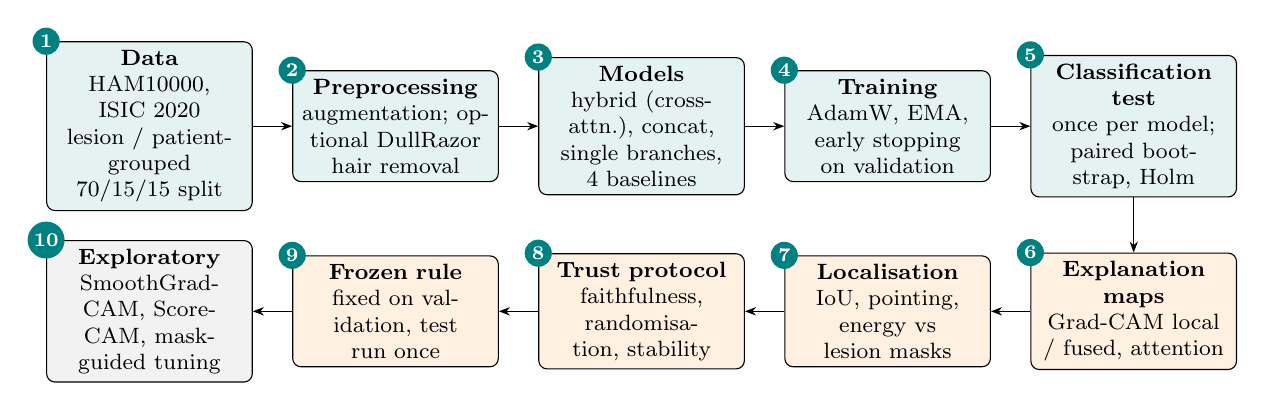
\begin{tikzpicture}[
    font=\footnotesize, >={Stealth[length=4pt]}, node distance=3mm and 5mm,
    wfbox/.style={draw, rounded corners=3pt, align=center, minimum height=13mm, text width=24mm, inner sep=3pt},
    wfnum/.style={circle, fill=secteal, text=white, font=\scriptsize\bfseries, inner sep=1.2pt},
    wfa/.style={wfbox, fill=teal!10},
    wfb/.style={wfbox, fill=orange!12},
    wfc/.style={wfbox, fill=gray!10},
]
  % row 1: classification
  \node[wfa] (s1) {\textbf{Data}\\HAM10000, ISIC 2020\\lesion / patient-grouped 70/15/15 split};
  \node[wfa, right=of s1] (s2) {\textbf{Preprocessing}\\augmentation; optional DullRazor hair removal};
  \node[wfa, right=of s2] (s3) {\textbf{Models}\\hybrid (cross-attn.), concat, single branches, 4 baselines};
  \node[wfa, right=of s3] (s4) {\textbf{Training}\\AdamW, EMA, early stopping on validation};
  \node[wfa, right=of s4] (s5) {\textbf{Classification test}\\once per model; paired bootstrap, Holm};
  % row 2: explanations
  \node[wfb, below=7mm of s5] (s6) {\textbf{Explanation maps}\\Grad-CAM local / fused, attention};
  \node[wfb, left=of s6] (s7) {\textbf{Localisation}\\IoU, pointing, energy vs lesion masks};
  \node[wfb, left=of s7] (s8) {\textbf{Trust protocol}\\faithfulness, randomisation, stability};
  \node[wfb, left=of s8] (s9) {\textbf{Frozen rule}\\fixed on validation, test run once};
  \node[wfc, left=of s9] (s10) {\textbf{Exploratory}\\SmoothGrad-CAM, Score-CAM, mask-guided tuning};

  \draw[->] (s1) -- (s2);
  \draw[->] (s2) -- (s3);
  \draw[->] (s3) -- (s4);
  \draw[->] (s4) -- (s5);
  \draw[->] (s5) -- (s6);
  \draw[->] (s6) -- (s7);
  \draw[->] (s7) -- (s8);
  \draw[->] (s8) -- (s9);
  \draw[->] (s9) -- (s10);
  \node[wfnum] at (s1.north west) {1};
  \node[wfnum] at (s2.north west) {2};
  \node[wfnum] at (s3.north west) {3};
  \node[wfnum] at (s4.north west) {4};
  \node[wfnum] at (s5.north west) {5};
  \node[wfnum] at (s6.north west) {6};
  \node[wfnum] at (s7.north west) {7};
  \node[wfnum] at (s8.north west) {8};
  \node[wfnum] at (s9.north west) {9};
  \node[wfnum] at (s10.north west) {10};
\end{tikzpicture}
.
% Style names avoid TikZ's own keys (the earlier "step" clashed with the grid key and the figure did not render).
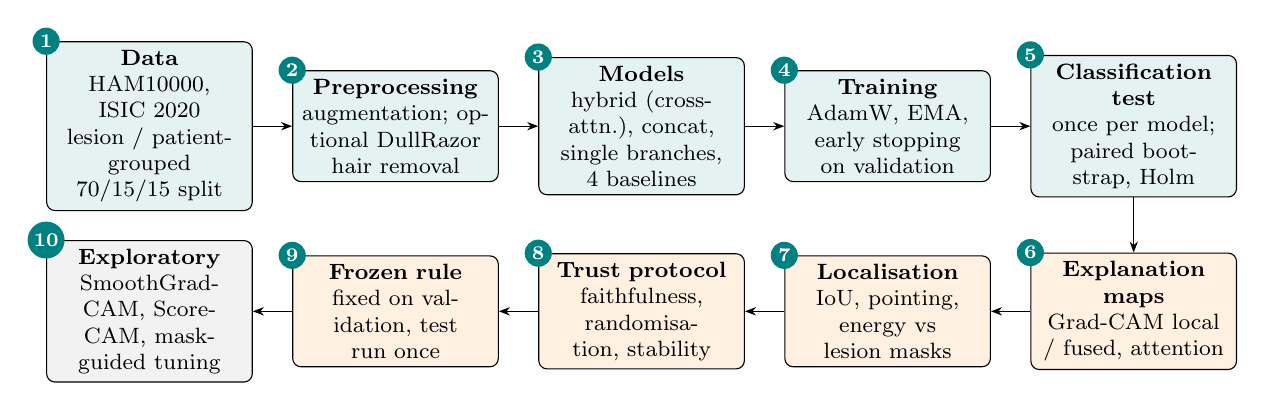
\begin{tikzpicture}[
    font=\footnotesize, >={Stealth[length=4pt]}, node distance=3mm and 5mm,
    wfbox/.style={draw, rounded corners=3pt, align=center, minimum height=13mm, text width=24mm, inner sep=3pt},
    wfnum/.style={circle, fill=secteal, text=white, font=\scriptsize\bfseries, inner sep=1.2pt},
    wfa/.style={wfbox, fill=teal!10},
    wfb/.style={wfbox, fill=orange!12},
    wfc/.style={wfbox, fill=gray!10},
]
  % row 1: classification
  \node[wfa] (s1) {\textbf{Data}\\HAM10000, ISIC 2020\\lesion / patient-grouped 70/15/15 split};
  \node[wfa, right=of s1] (s2) {\textbf{Preprocessing}\\augmentation; optional DullRazor hair removal};
  \node[wfa, right=of s2] (s3) {\textbf{Models}\\hybrid (cross-attn.), concat, single branches, 4 baselines};
  \node[wfa, right=of s3] (s4) {\textbf{Training}\\AdamW, EMA, early stopping on validation};
  \node[wfa, right=of s4] (s5) {\textbf{Classification test}\\once per model; paired bootstrap, Holm};
  % row 2: explanations
  \node[wfb, below=7mm of s5] (s6) {\textbf{Explanation maps}\\Grad-CAM local / fused, attention};
  \node[wfb, left=of s6] (s7) {\textbf{Localisation}\\IoU, pointing, energy vs lesion masks};
  \node[wfb, left=of s7] (s8) {\textbf{Trust protocol}\\faithfulness, randomisation, stability};
  \node[wfb, left=of s8] (s9) {\textbf{Frozen rule}\\fixed on validation, test run once};
  \node[wfc, left=of s9] (s10) {\textbf{Exploratory}\\SmoothGrad-CAM, Score-CAM, mask-guided tuning};

  \draw[->] (s1) -- (s2);
  \draw[->] (s2) -- (s3);
  \draw[->] (s3) -- (s4);
  \draw[->] (s4) -- (s5);
  \draw[->] (s5) -- (s6);
  \draw[->] (s6) -- (s7);
  \draw[->] (s7) -- (s8);
  \draw[->] (s8) -- (s9);
  \draw[->] (s9) -- (s10);
  \node[wfnum] at (s1.north west) {1};
  \node[wfnum] at (s2.north west) {2};
  \node[wfnum] at (s3.north west) {3};
  \node[wfnum] at (s4.north west) {4};
  \node[wfnum] at (s5.north west) {5};
  \node[wfnum] at (s6.north west) {6};
  \node[wfnum] at (s7.north west) {7};
  \node[wfnum] at (s8.north west) {8};
  \node[wfnum] at (s9.north west) {9};
  \node[wfnum] at (s10.north west) {10};
\end{tikzpicture}
.
% Style names avoid TikZ's own keys (the earlier "step" clashed with the grid key and the figure did not render).
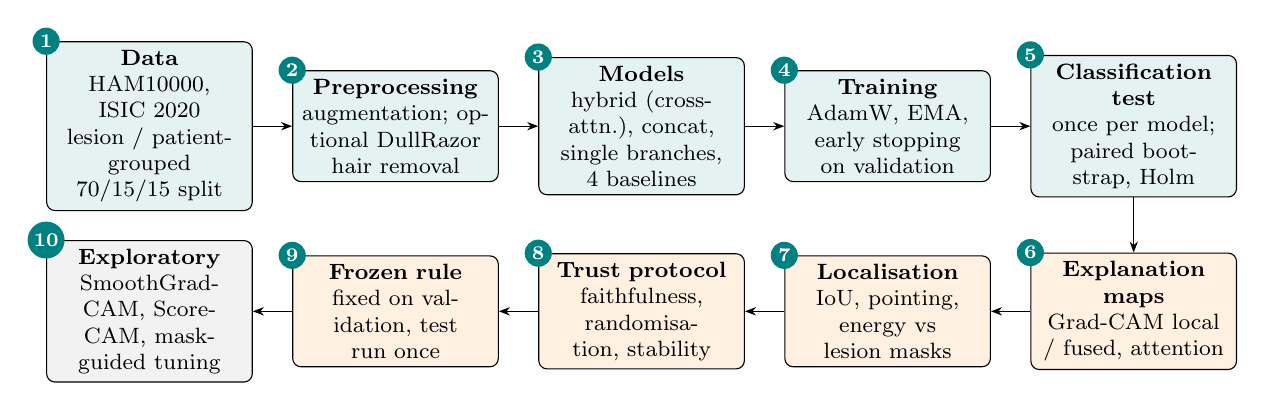
\begin{tikzpicture}[
    font=\footnotesize, >={Stealth[length=4pt]}, node distance=3mm and 5mm,
    wfbox/.style={draw, rounded corners=3pt, align=center, minimum height=13mm, text width=24mm, inner sep=3pt},
    wfnum/.style={circle, fill=secteal, text=white, font=\scriptsize\bfseries, inner sep=1.2pt},
    wfa/.style={wfbox, fill=teal!10},
    wfb/.style={wfbox, fill=orange!12},
    wfc/.style={wfbox, fill=gray!10},
]
  % row 1: classification
  \node[wfa] (s1) {\textbf{Data}\\HAM10000, ISIC 2020\\lesion / patient-grouped 70/15/15 split};
  \node[wfa, right=of s1] (s2) {\textbf{Preprocessing}\\augmentation; optional DullRazor hair removal};
  \node[wfa, right=of s2] (s3) {\textbf{Models}\\hybrid (cross-attn.), concat, single branches, 4 baselines};
  \node[wfa, right=of s3] (s4) {\textbf{Training}\\AdamW, EMA, early stopping on validation};
  \node[wfa, right=of s4] (s5) {\textbf{Classification test}\\once per model; paired bootstrap, Holm};
  % row 2: explanations
  \node[wfb, below=7mm of s5] (s6) {\textbf{Explanation maps}\\Grad-CAM local / fused, attention};
  \node[wfb, left=of s6] (s7) {\textbf{Localisation}\\IoU, pointing, energy vs lesion masks};
  \node[wfb, left=of s7] (s8) {\textbf{Trust protocol}\\faithfulness, randomisation, stability};
  \node[wfb, left=of s8] (s9) {\textbf{Frozen rule}\\fixed on validation, test run once};
  \node[wfc, left=of s9] (s10) {\textbf{Exploratory}\\SmoothGrad-CAM, Score-CAM, mask-guided tuning};

  \draw[->] (s1) -- (s2);
  \draw[->] (s2) -- (s3);
  \draw[->] (s3) -- (s4);
  \draw[->] (s4) -- (s5);
  \draw[->] (s5) -- (s6);
  \draw[->] (s6) -- (s7);
  \draw[->] (s7) -- (s8);
  \draw[->] (s8) -- (s9);
  \draw[->] (s9) -- (s10);
  \node[wfnum] at (s1.north west) {1};
  \node[wfnum] at (s2.north west) {2};
  \node[wfnum] at (s3.north west) {3};
  \node[wfnum] at (s4.north west) {4};
  \node[wfnum] at (s5.north west) {5};
  \node[wfnum] at (s6.north west) {6};
  \node[wfnum] at (s7.north west) {7};
  \node[wfnum] at (s8.north west) {8};
  \node[wfnum] at (s9.north west) {9};
  \node[wfnum] at (s10.north west) {10};
\end{tikzpicture}
}
\caption{Overall workflow of the study. Steps 1--5 cover classification, steps 6--9 the confirmatory explanation
analysis, and step 10 the exploratory follow-ups.}
\label{fig:workflow}
\end{figure*}

\subsection{Datasets}
HAM10000 \cite{tschandl2018ham10000} contains 10,015 dermoscopic images of 7,470 lesions in seven classes (actinic
keratosis \textit{akiec}, basal cell carcinoma \textit{bcc}, benign keratosis \textit{bkl}, dermatofibroma
\textit{df}, melanoma \textit{mel}, melanocytic nevus \textit{nv}, vascular lesion \textit{vasc}). The original
$600\times450$ images are used, together with the expert lesion segmentation that is publicly available for every
image. ISIC 2020 \cite{rotemberg2021isic2020} is used through a public copy resized to
$256\times256$ (33,126 images, 2,056 patients, 584 melanomas, 1.76\%). Its official test labels are not public, so the
public training set is split here, and the task is melanoma versus benign. ISIC 2020 has no lesion masks.

Both datasets are split 70/15/15 with class stratification. Because HAM10000 has 10,015 images of only 7,470 lesions,
the split is grouped by lesion, and ISIC 2020 is grouped by patient, so that no lesion or patient appears in two
splits (Table~\ref{tab:splits}). The split files are written once with a fixed seed and read by every run. The
validation split is used for model selection and for fixing every evaluation setting; each test split is used once
per model.

\begin{table}[!t]
\centering
\caption{Images per Class and Split}
\label{tab:splits}
% Generated by scripts/make_report_tables.py; do not edit by hand.
% Sources: data/splits/ham10000_summary.csv, data/splits/isic2020_summary.csv
\small
\setlength{\tabcolsep}{3pt}
\renewcommand{\arraystretch}{1.1}
\begin{tabularx}{\columnwidth}{|>{\raggedright\arraybackslash}X|r|r|r|}
\hline
\textbf{Class} & \textbf{Train} & \textbf{Val} & \textbf{Test} \\ \hline
\multicolumn{4}{|l|}{\textit{HAM10000 (grouped by lesion)}} \\
\hline
akiec & 228 & 50 & 49 \\
bcc & 359 & 77 & 78 \\
bkl & 769 & 165 & 165 \\
df & 80 & 18 & 17 \\
mel & 779 & 166 & 168 \\
nv & 4{,}694 & 1{,}006 & 1{,}005 \\
vasc & 100 & 21 & 21 \\
\textit{total images} & 7{,}009 & 1{,}503 & 1{,}503 \\
\textit{groups (lesions/patients)} & 5{,}230 & 1{,}122 & 1{,}118 \\
\hline
\multicolumn{4}{|l|}{\textit{ISIC 2020 (grouped by patient)}} \\
\hline
benign & 22{,}782 & 4{,}882 & 4{,}878 \\
melanoma & 408 & 87 & 89 \\
\textit{total images} & 23{,}190 & 4{,}969 & 4{,}967 \\
\textit{groups (lesions/patients)} & 1{,}440 & 309 & 307 \\
\hline
\end{tabularx}

\end{table}

\subsection{Preprocessing and Data Augmentation}
During training, images are randomly resized and cropped to $224\times224$ (scale 0.7--1.0), flipped, rotated by
multiples of $90^\circ$, slightly translated, scaled and rotated, and colour-jittered. At evaluation the shorter side
is resized and the centre is cropped to $224\times224$. The hybrid gives each branch the input normalisation its
backbone was pretrained with (Section~\ref{sec:baselines} describes two baselines first trained without it).

For an ablation, hair is removed with a simplified version of the DullRazor algorithm: black-hat morphology, a
threshold, a test that keeps only long and thin regions, and Telea inpainting. A visual check of 100 images showed
failure cases in which thin lesion borders or pigment network were removed as hair.

\subsection{Proposed Architecture}
Fig.~\ref{fig:arch} shows the hybrid model (55.61 million parameters).

\begin{figure*}[!t]
\centering
\resizebox{0.95\textwidth}{!}{% F0: architecture of the hybrid (drawn by hand; dimensions from configs/model/hybrid.yaml and models/fusion.py).
% Used inside a figure* in main.tex via % F0: architecture of the hybrid (drawn by hand; dimensions from configs/model/hybrid.yaml and models/fusion.py).
% Used inside a figure* in main.tex via % F0: architecture of the hybrid (drawn by hand; dimensions from configs/model/hybrid.yaml and models/fusion.py).
% Used inside a figure* in main.tex via \input{figures/f0_architecture}.
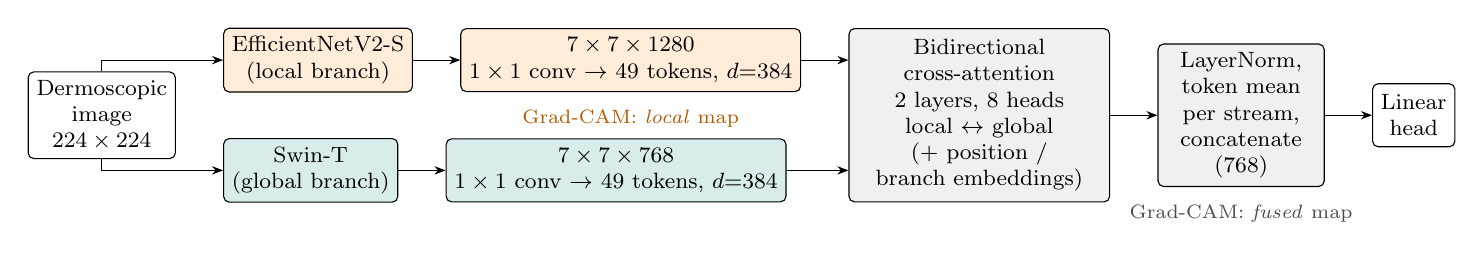
\begin{tikzpicture}[
    font=\footnotesize, >={Stealth[length=4pt]}, node distance=4mm and 6mm,
    box/.style={draw, rounded corners=2pt, align=center, minimum height=8mm, inner sep=3pt},
    loc/.style={box, fill=orange!15},
    glo/.style={box, fill=teal!15},
    fus/.style={box, fill=gray!12},
]
  \node[box] (img) {Dermoscopic\\image\\$224\times224$};
  \node[loc, right=of img, yshift=7mm]  (eff) {EfficientNetV2-S\\(local branch)};
  \node[glo, right=of img, yshift=-7mm] (swin) {Swin-T\\(global branch)};
  \node[loc, right=of eff]  (lgrid) {$7\times7\times1280$\\$1\times1$ conv $\rightarrow$ 49 tokens, $d{=}384$};
  \node[glo, right=of swin] (ggrid) {$7\times7\times768$\\$1\times1$ conv $\rightarrow$ 49 tokens, $d{=}384$};
  \node[fus, right=of lgrid, yshift=-7mm, minimum height=22mm, text width=31mm] (fusion)
       {Bidirectional cross-attention\\$2$ layers, $8$ heads\\local $\leftrightarrow$ global\\(+ position / branch embeddings)};
  \node[fus, right=of fusion, text width=19mm] (pool) {LayerNorm,\\token mean per stream,\\concatenate (768)};
  \node[box, right=of pool] (head) {Linear\\head};

  \draw[->] (img) |- (eff);
  \draw[->] (img) |- (swin);
  \draw[->] (eff) -- (lgrid);
  \draw[->] (swin) -- (ggrid);
  \draw[->] (lgrid.east) -- (lgrid.east -| fusion.west);
  \draw[->] (ggrid.east) -- (ggrid.east -| fusion.west);
  \draw[->] (fusion) -- (pool);
  \draw[->] (pool) -- (head);

  \node[below=1mm of lgrid.south, font=\scriptsize, text=orange!70!black] {Grad-CAM: \emph{local} map};
  \node[below=1mm of pool.south, font=\scriptsize, text=gray!60!black, align=center] {Grad-CAM: \emph{fused} map};
\end{tikzpicture}
.
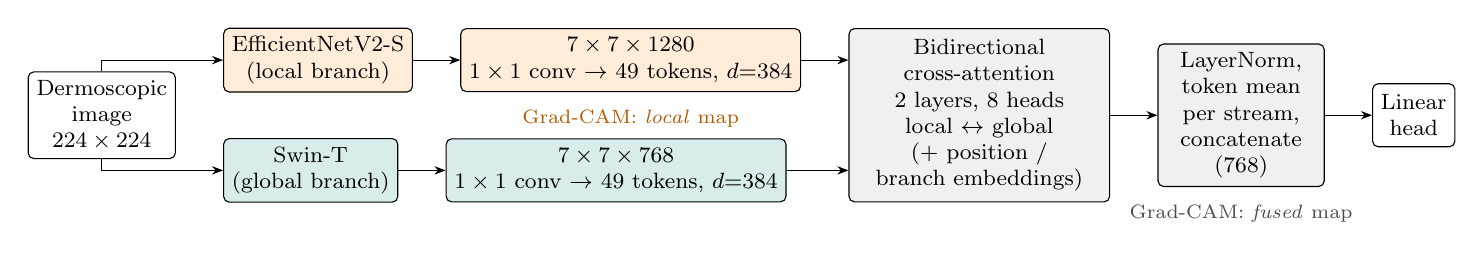
\begin{tikzpicture}[
    font=\footnotesize, >={Stealth[length=4pt]}, node distance=4mm and 6mm,
    box/.style={draw, rounded corners=2pt, align=center, minimum height=8mm, inner sep=3pt},
    loc/.style={box, fill=orange!15},
    glo/.style={box, fill=teal!15},
    fus/.style={box, fill=gray!12},
]
  \node[box] (img) {Dermoscopic\\image\\$224\times224$};
  \node[loc, right=of img, yshift=7mm]  (eff) {EfficientNetV2-S\\(local branch)};
  \node[glo, right=of img, yshift=-7mm] (swin) {Swin-T\\(global branch)};
  \node[loc, right=of eff]  (lgrid) {$7\times7\times1280$\\$1\times1$ conv $\rightarrow$ 49 tokens, $d{=}384$};
  \node[glo, right=of swin] (ggrid) {$7\times7\times768$\\$1\times1$ conv $\rightarrow$ 49 tokens, $d{=}384$};
  \node[fus, right=of lgrid, yshift=-7mm, minimum height=22mm, text width=31mm] (fusion)
       {Bidirectional cross-attention\\$2$ layers, $8$ heads\\local $\leftrightarrow$ global\\(+ position / branch embeddings)};
  \node[fus, right=of fusion, text width=19mm] (pool) {LayerNorm,\\token mean per stream,\\concatenate (768)};
  \node[box, right=of pool] (head) {Linear\\head};

  \draw[->] (img) |- (eff);
  \draw[->] (img) |- (swin);
  \draw[->] (eff) -- (lgrid);
  \draw[->] (swin) -- (ggrid);
  \draw[->] (lgrid.east) -- (lgrid.east -| fusion.west);
  \draw[->] (ggrid.east) -- (ggrid.east -| fusion.west);
  \draw[->] (fusion) -- (pool);
  \draw[->] (pool) -- (head);

  \node[below=1mm of lgrid.south, font=\scriptsize, text=orange!70!black] {Grad-CAM: \emph{local} map};
  \node[below=1mm of pool.south, font=\scriptsize, text=gray!60!black, align=center] {Grad-CAM: \emph{fused} map};
\end{tikzpicture}
.
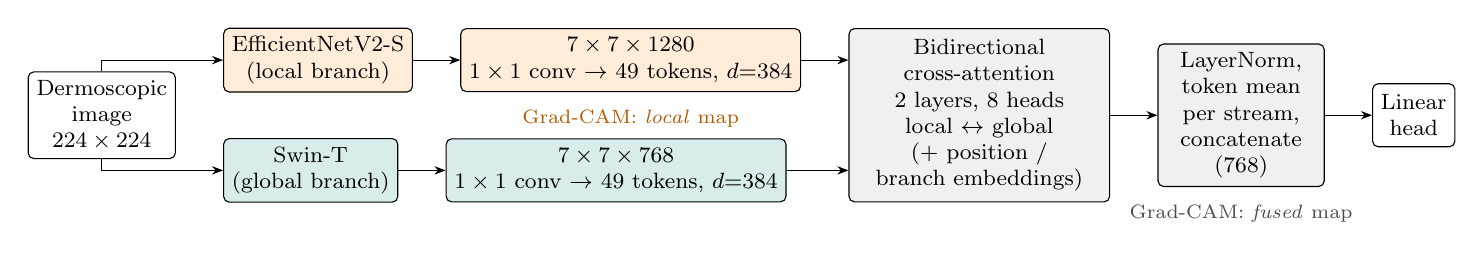
\begin{tikzpicture}[
    font=\footnotesize, >={Stealth[length=4pt]}, node distance=4mm and 6mm,
    box/.style={draw, rounded corners=2pt, align=center, minimum height=8mm, inner sep=3pt},
    loc/.style={box, fill=orange!15},
    glo/.style={box, fill=teal!15},
    fus/.style={box, fill=gray!12},
]
  \node[box] (img) {Dermoscopic\\image\\$224\times224$};
  \node[loc, right=of img, yshift=7mm]  (eff) {EfficientNetV2-S\\(local branch)};
  \node[glo, right=of img, yshift=-7mm] (swin) {Swin-T\\(global branch)};
  \node[loc, right=of eff]  (lgrid) {$7\times7\times1280$\\$1\times1$ conv $\rightarrow$ 49 tokens, $d{=}384$};
  \node[glo, right=of swin] (ggrid) {$7\times7\times768$\\$1\times1$ conv $\rightarrow$ 49 tokens, $d{=}384$};
  \node[fus, right=of lgrid, yshift=-7mm, minimum height=22mm, text width=31mm] (fusion)
       {Bidirectional cross-attention\\$2$ layers, $8$ heads\\local $\leftrightarrow$ global\\(+ position / branch embeddings)};
  \node[fus, right=of fusion, text width=19mm] (pool) {LayerNorm,\\token mean per stream,\\concatenate (768)};
  \node[box, right=of pool] (head) {Linear\\head};

  \draw[->] (img) |- (eff);
  \draw[->] (img) |- (swin);
  \draw[->] (eff) -- (lgrid);
  \draw[->] (swin) -- (ggrid);
  \draw[->] (lgrid.east) -- (lgrid.east -| fusion.west);
  \draw[->] (ggrid.east) -- (ggrid.east -| fusion.west);
  \draw[->] (fusion) -- (pool);
  \draw[->] (pool) -- (head);

  \node[below=1mm of lgrid.south, font=\scriptsize, text=orange!70!black] {Grad-CAM: \emph{local} map};
  \node[below=1mm of pool.south, font=\scriptsize, text=gray!60!black, align=center] {Grad-CAM: \emph{fused} map};
\end{tikzpicture}
}
\caption{Architecture of the hybrid model. Both $7\times7$ feature grids become 49 tokens that exchange information
in two bidirectional cross-attention layers; the local and fused Grad-CAM maps are taken where marked.}
\label{fig:arch}
\end{figure*}

\subsubsection{Backbone Selection Rationale}
The two branches are chosen to be complementary and comparable. EfficientNetV2-S \cite{tan2021efficientnetv2} is a
CNN that keeps fine local texture, and Swin-T \cite{liu2021swin} is a hierarchical Transformer that models wider
context. Both end in a $7\times7$ grid at $224\times224$ input, so their positions can be matched token by token.
Both are also strong single models in their own right, so the hybrid can be compared with each branch trained alone.

\subsubsection{Local Branch}
An EfficientNetV2-S backbone (ImageNet-21k pretraining, fine-tuned on ImageNet-1k) produces a $7\times7\times1280$
feature grid that keeps fine texture.

\subsubsection{Global Branch}
A Swin-T backbone (ImageNet-22k pretraining, fine-tuned on ImageNet-1k) produces a $7\times7\times768$ grid whose
features are built with windowed self-attention across the image.

\subsubsection{Bidirectional Cross-Attention Fusion}
Each grid is projected to $d = 384$ channels by a $1\times1$ convolution and flattened into 49 tokens; a learned
position embedding and a branch embedding are added. In each of two fusion layers, the local tokens attend to the
global tokens and vice versa, using multi-head cross-attention with eight heads:
\begin{equation}
\mathrm{CA}(X, C) = \mathrm{softmax}\!\left(\frac{(XW_Q)(CW_K)^\top}{\sqrt{d_h}}\right)CW_V
\label{eq:ca}
\end{equation}
where:
\begin{itemize}
\item $X$ are the query tokens of one stream and $C$ the tokens of the other stream
\item $W_Q, W_K, W_V$ are learned projections and $d_h = d/8$ is the head dimension
\end{itemize}
Each layer is a pre-norm residual block, $X \leftarrow X + \mathrm{CA}(\mathrm{LN}(X), \mathrm{LN}(C))$ followed by
$X \leftarrow X + \mathrm{MLP}(\mathrm{LN}(X))$, applied to both streams at the same time.

\subsubsection{Classification Head}
After a final layer normalisation, the tokens of each stream are averaged and the two means are concatenated:
\begin{equation}
\mathbf{y} = W\left[\tfrac{1}{N}\textstyle\sum_{n} \mathrm{LN}(T^{L})_{n} \,;\, \tfrac{1}{N}\sum_{n}
\mathrm{LN}(T^{G})_{n}\right] + \mathbf{b}
\label{eq:head}
\end{equation}
where $T^{L}, T^{G}$ are the local and global token streams, $N = 49$, and $W$ is a linear layer initialised to zero.

\subsection{Baselines and Ablations}\label{sec:baselines}
The baselines are ResNet-50 \cite{he2016resnet}, ConvNeXt-T \cite{liu2022convnext}, ViT-B/16
\cite{dosovitskiy2021vit} and Swin-T \cite{liu2021swin}, all ImageNet-pretrained. The ablations are each branch
trained alone (EfficientNetV2-S and Swin-T), the same two branches fused by concatenating their average-pooled
features into one vector (47.71 million parameters; no attention between the branches), and the hybrid and
ConvNeXt-T trained on hair-removed images. EfficientNetV2-S and ViT-B/16 were first trained with ImageNet
normalisation instead of their pretrained normalisation; both were retrained with the correct normalisation, and
both versions are reported.

\subsection{Optimisation and Training}
All models share one recipe (Table~\ref{tab:training}) with the AdamW optimiser, a short warm-up followed by
cosine decay, mixed precision, gradient clipping and early stopping on validation, adapted from GC-ViT-E
(Sec.~3.4) \cite{alhaj2026gcvite} and the ViT fine-tuning setup (ViT, App.~B.1.1) \cite{dosovitskiy2021vit}. The loss is a class-weighted cross-entropy with label smoothing:
\begin{equation}
\mathcal{L}_{\mathrm{CE}} = -\sum_{c=1}^{K} w_{y}\, q_c \log p_c, \qquad
q_c = (1-\varepsilon)\,\mathbb{1}[c = y] + \tfrac{\varepsilon}{K}
\label{eq:loss}
\end{equation}
where:
\begin{itemize}
\item $p_c$ is the predicted probability of class $c$ and $y$ the true class
\item $w_y \propto n_y^{-1/2}$ is the weight of class $y$ with $n_y$ training images
\item $\varepsilon = 0.1$ is the label smoothing and $K$ the number of classes
\end{itemize}
The checkpoint with the best validation macro-F1 (HAM10000) or AUC (ISIC 2020) of the exponential moving average of
the weights is kept. ViT-B/16 needed a lower backbone learning rate ($3\times10^{-5}$), chosen after one validation
run; this is the only model-specific change.

\begin{table}[!t]
\centering
\caption{Training Configuration}
\label{tab:training}
% Generated by scripts/make_report_tables.py; do not edit by hand.
% Sources: configs/data/ham10000.yaml, configs/model/hybrid.yaml, configs/train/default.yaml, configs/train/kaggle_16gb.yaml, configs/train/local_4gb.yaml, configs/train/mask_finetune.yaml
\small
\setlength{\tabcolsep}{3pt}
\renewcommand{\arraystretch}{1.1}
\begin{tabularx}{\columnwidth}{|>{\raggedright\arraybackslash}X|>{\raggedright\arraybackslash}X|}
\hline
\textbf{Setting} & \textbf{Value} \\ \hline
\multicolumn{2}{|l|}{\textit{Optimisation (all models)}} \\
\hline
Optimiser & AdamW \\
Learning rate, backbone / fusion + head & $1\times10^{-4}$ / $1\times10^{-3}$ \\
Weight decay & $0.05$ \\
Schedule & 3 warm-up epochs, cosine to 0.01$\times$ \\
Maximum epochs; early stopping & 30; patience 7 on val macro-F1 (AUC on ISIC) \\
Loss & cross-entropy, label smoothing 0.1, class weights (1/freq)$^{0.5}$ \\
Gradient clipping; EMA decay & 1.0; 0.999 \\
Mixed precision; seed & yes; 42 \\
Input size & $224\times224$ \\
\hline
\multicolumn{2}{|l|}{\textit{Hardware profiles}} \\
\hline
Local (RTX 3050, 4 GB) & batch 8 $\times$ 4 accumulation, gradient checkpointing \\
Kaggle (ISIC 2020) & batch 32, no accumulation \\
\hline
\multicolumn{2}{|l|}{\textit{Hybrid fusion}} \\
\hline
Token dimension; layers; heads & 384; 2; 8 \\
Dropout; drop path & 0.2; 0.1 \\
\hline
\multicolumn{2}{|l|}{\textit{Mask-guided fine-tuning (exploratory)}} \\
\hline
Epochs; learning rates & 5; $1\times10^{-5}$ / $1\times10^{-4}$, no warm-up \\
\hline
\end{tabularx}

\end{table}

\subsection{Explanation Maps}
Grad-CAM \cite{selvaraju2020gradcam} computes, for class $c$ and feature maps $A^k$ of a layer (Grad-CAM, Sec.~3,
Eq.~1--2):
\begin{equation}
\alpha_k^c = \frac{1}{Z}\sum_{i,j}\frac{\partial y^c}{\partial A^k_{ij}}, \qquad
L^c = \mathrm{ReLU}\Big(\sum_k \alpha_k^c A^k\Big)
\label{eq:gradcam}
\end{equation}
where $y^c$ is the score of class $c$ before the softmax and $Z$ the number of spatial positions. Maps are computed
for the predicted class on the $7\times7$ grids and upsampled to $224\times224$.

The \textit{local} map uses the EfficientNetV2-S grid of the hybrid. The \textit{fused} map uses the two normalised
token streams of the fusion, which share the same $7\times7$ positions, and sums their contributions. Because the
head in Eq.~(\ref{eq:head}) is linear in the token means, the gradient of $y^c$ with respect to a token is
$W_{c,k}/N$, and the fused Grad-CAM equals the class activation map \cite{zhou2016cam} scaled by $1/N$:
\begin{equation}
L^c_{\mathrm{fused}} = \frac{1}{N}\,\mathrm{ReLU}\Big(\sum_k W_{c,k}\big(\mathrm{LN}(T^{L})_{k} +
\mathrm{LN}(T^{G})_{k}\big)\Big)
\label{eq:fused}
\end{equation}
ConvNeXt-T maps use its last stage. Attention rollout and the cross-attention maps are computed as additional,
class-agnostic maps.

\subsection{Explanation Trust Protocol}
The question ``is a hybrid map more trustworthy than ConvNeXt-T's Grad-CAM?'' is answered with four properties,
each measured per image and averaged.

\subsubsection{Localisation}
A map is binarised at 15\% of its maximum (Grad-CAM, Sec.~4.1) and compared with the lesion mask $M$:
\begin{equation}
\mathrm{IoU} = \frac{|B \cap M|}{|B \cup M|}, \qquad B = \{p : L(p) \geq 0.15 \max L\}
\label{eq:iou}
\end{equation}
The pointing game (Grad-CAM, Sec.~4.3) checks whether the maximum of the map lies in the lesion, and the energy in
mask is the share of the map's total value inside it. The IoU gap is the mean IoU on correctly classified images
minus that on misclassified ones; a trustworthy explanation should be worse when the model is wrong. A centred
Gaussian map and a uniform map serve as input-independent references.

\subsubsection{Faithfulness}
Pixels are ranked by the map and removed (deletion: replaced by the dataset-mean colour) or restored into a blurred
image (insertion) in 50 steps, while the probability of the predicted class is recorded \cite{petsiuk2018rise}.
Each curve gives an area under the curve (AUC). Because the two models' probabilities on fully deleted images
differ, the endpoint is the difference to a random map:
\begin{equation}
\Delta_{\mathrm{del}} = \mathrm{AUC}_{\mathrm{del}}(L) - \mathrm{AUC}_{\mathrm{del}}(R), \qquad
\Delta_{\mathrm{ins}} = \mathrm{AUC}_{\mathrm{ins}}(L) - \mathrm{AUC}_{\mathrm{ins}}(R)
\label{eq:faith}
\end{equation}
where $R$ is uniform noise on a $7\times7$ grid upsampled like the real maps. Lower $\Delta_{\mathrm{del}}$ and
higher $\Delta_{\mathrm{ins}}$ are better.

\subsubsection{Parameter Randomisation}
Following Adebayo et al. \cite{adebayo2018sanity}, the model's blocks are re-initialised from the head downwards
until every block is random. The structural similarity (SSIM) between the trained and the fully randomised map is
the endpoint (lower is better); absolute rank correlations are reported next to it.

\subsubsection{Stability}
The input is flipped, given Gaussian noise ($\sigma = 0.03$), or brightened or darkened by 10\%. The Spearman
correlation between the original and the perturbed map (flipped back where needed) is averaged over the
perturbations that leave the prediction unchanged (higher is better).

\subsubsection{Primary Endpoints and Decision Rule}
For each of the two hybrid maps, six primary endpoints are tested: $\Delta_{\mathrm{del}}$, $\Delta_{\mathrm{ins}}$,
randomisation SSIM, stability, IoU and IoU gap (12 tests, Holm-corrected together). A hybrid map counts as more
trustworthy than ConvNeXt-T's Grad-CAM only if, with Holm-adjusted $p < 0.05$,
\begin{equation}
\big(\Delta_{\mathrm{del}}\!\uparrow \lor \Delta_{\mathrm{ins}}\!\uparrow\big) \land
\mathrm{SSIM}_{\mathrm{rand}}\!\uparrow \land \neg\,\exists\, e \in E : e\!\downarrow
\label{eq:rule}
\end{equation}
where $\uparrow$ / $\downarrow$ denote a significant improvement / deterioration and $E$ is the set of primary
endpoints. The protocol was frozen on the validation set, where four documented changes were made (the
random-map baseline in Eq.~(\ref{eq:faith}), the unchanged-prediction rule for stability, the SSIM caveat, and
absolute values for the exploratory rank correlations). The test set was then evaluated once.

\subsection{Statistical Analysis}
All comparisons are paired: both models are evaluated on the same 1,000 bootstrap resamples of the test images.
For a difference $d = B - A$, the 95\% confidence interval is the 2.5th--97.5th percentile
of the resampled differences, and the two-sided p-value is
\begin{equation}
p = 2\min\big(P^*(d^* \leq 0),\, P^*(d^* \geq 0)\big)
\label{eq:pval}
\end{equation}
where $P^*$ is the share of resamples. With 1,000 resamples the smallest non-zero value is 0.002; a value of zero is
reported as $p < 0.002$. Within a family of $m$ tests, Holm's step-down method adjusts the ordered p-values
$p_{(1)} \leq \dots \leq p_{(m)}$ to
\begin{equation}
\tilde p_{(i)} = \max_{j \leq i} \min\big(1, (m - j + 1)\, p_{(j)}\big)
\label{eq:holm}
\end{equation}
so a raw $p < 0.002$ becomes $\tilde p < 0.024$ in the 12-test explanation family. For classification, the primary
endpoint is macro-F1 with Holm correction over two pre-specified comparisons (hybrid versus ConvNeXt-T, and hybrid
versus concatenation). On ISIC 2020, two decision cutoffs are fixed on the validation set before the test run: the
Youden cutoff and the highest cutoff with validation sensitivity $\geq 0.80$.

\subsection{Exploratory Follow-ups}
After the confirmatory test, three follow-ups ask whether the explanations can be made more trustworthy. Because
the HAM10000 test set had already been used, they are \textit{exploratory}, although their settings and decision
rules were again fixed on validation first.

\subsubsection{SmoothGrad-CAM}
Grad-CAM is averaged over 50 noisy copies of the input with noise standard deviation $0.15$ times the input range,
the settings of the sanity-check code \cite{adebayo2018sanity, smilkov2017smoothgrad}.

\subsubsection{Score-CAM}
Each channel, upsampled and scaled to $[0,1]$, masks the input; its weight is the softmax probability of the target
class for that masked input (Score-CAM). Because this needs one forward pass per channel, Score-CAM is
run on a fixed stratified subset of 150 images per split.

\subsubsection{Mask-Guided Fine-Tuning}
The hybrid is fine-tuned with lesion masks from the training split so that its fused map, Eq.~(\ref{eq:fused}),
stays inside the lesion:
\begin{equation}
\mathcal{L} = \mathcal{L}_{\mathrm{CE}} + \lambda\,\frac{\sum_p L(p)\,(1 - m(p))}{\sum_p L(p)} +
\mu\,\big(1 - \cos(L, L_{\mathrm{noise}})\big)
\label{eq:mask}
\end{equation}
where $m$ is the lesion mask pooled to $7\times7$ and $L_{\mathrm{noise}}$ the map of a noisy copy of the image. This
follows the idea of constraining an explanation map during training. Five candidates
($\lambda \in \{0.1, 0.3, 1\}$, then $\mu \in \{0.1, 1\}$) were screened on validation; a candidate was eligible only
if its validation macro-F1 stayed within 0.01 of the original model.

% =================================================================================================== 4
\section{Experimental Results and Performance Evaluation}
This section reports the classification results on both datasets, the localisation of the explanation maps, the
confirmatory explanation-trust test and the exploratory follow-ups. All test numbers come from a single evaluation
per model.

\subsection{Experimental Setup}
Experiments were run on the following hardware and software:
\begin{itemize}
\item HAM10000: one NVIDIA RTX 3050 laptop GPU (4 GB) with 7.3 GB system memory
\item ISIC 2020: Kaggle sessions with two NVIDIA Tesla T4 GPUs
\item Python 3.11, PyTorch 2.6, timm 1.0.30, albumentations 2.0.8, scikit-learn 1.9.1, OpenCV and scikit-image
\item PyCharm for development and Overleaf for the report
\end{itemize}
Training the hybrid on HAM10000 took 17 epochs (best at epoch 10) and about 4 hours on the local GPU.

\subsection{Evaluation Metrics}

\subsubsection{Accuracy and Balanced Accuracy}
\begin{equation}
\mathrm{Accuracy} = \frac{TP + TN}{TP + TN + FP + FN}, \qquad \mathrm{BA} = \frac{1}{K}\sum_{c=1}^{K}\mathrm{Recall}_c
\label{eq:acc}
\end{equation}
where $TP$, $TN$, $FP$ and $FN$ are true and false positives and negatives. Balanced accuracy (BA) averages the
recall of each class and is not dominated by the majority class \textit{nv}.

\subsubsection{Precision, Recall and Macro-F1}
\begin{equation}
\mathrm{F1}_c = \frac{2\,\mathrm{Precision}_c\,\mathrm{Recall}_c}{\mathrm{Precision}_c + \mathrm{Recall}_c},
\qquad \mathrm{F1}_{\mathrm{macro}} = \frac{1}{K}\sum_{c=1}^{K}\mathrm{F1}_c
\label{eq:f1}
\end{equation}
with $\mathrm{Precision}_c = TP_c/(TP_c + FP_c)$ and $\mathrm{Recall}_c = TP_c/(TP_c + FN_c)$. Macro-F1 is the
model-selection metric and the primary classification endpoint on HAM10000; the recall of melanoma is reported as
melanoma sensitivity.

\subsubsection{Matthews Correlation Coefficient}
The multiclass MCC summarises the whole confusion matrix in one value between $-1$ and $1$ and is robust to class
imbalance.

\subsubsection{AUC and Average Precision}
The area under the ROC curve (AUC; one-versus-rest macro average on HAM10000) measures ranking. On ISIC 2020, with
1.76\% melanoma, average precision (AP), the area under the precision--recall curve, shows how many positive calls
are correct.

\subsection{HAM10000 Classification}
Table~\ref{tab:ham} lists all HAM10000 runs. ConvNeXt-T is the strongest model that was planned for comparison
(test macro-F1 0.8118 [0.7775, 0.8424]). The cross-attention hybrid reaches 0.7903 [0.7501, 0.8260], close to the
concatenation hybrid (0.7823) and above its own branches trained alone (EfficientNetV2-S with pretrained
normalisation 0.7655, Swin-T 0.7710). ResNet-50 is clearly the weakest (0.7111).

\begin{table*}[!t]
\centering
\caption{HAM10000 Test Classification (n = 1,503; 95\% Bootstrap CI). Val F1: Best-Epoch Validation Macro-F1.
$^a$ImageNet Instead of Pretrained Input Normalisation. $^b$Not a Pre-Specified Comparison.
\textsuperscript{\textdagger}Exploratory. Best Value per Column in Bold}
\label{tab:ham}
% Generated by scripts/make_report_tables.py; do not edit by hand.
% Sources: outputs/runs/ham10000_convnext_t/eval/metrics.json, outputs/runs/ham10000_convnext_t/train_summary.json, outputs/runs/ham10000_convnext_t_hair/eval/metrics.json, outputs/runs/ham10000_convnext_t_hair/train_summary.json, outputs/runs/ham10000_effnetv2_s/eval/metrics.json, outputs/runs/ham10000_effnetv2_s/train_summary.json, outputs/runs/ham10000_effnetv2_s_pnorm/eval/metrics.json, outputs/runs/ham10000_effnetv2_s_pnorm/train_summary.json, outputs/runs/ham10000_hybrid/eval/metrics.json, outputs/runs/ham10000_hybrid/train_summary.json, outputs/runs/ham10000_hybrid_concat/eval/metrics.json, outputs/runs/ham10000_hybrid_concat/train_summary.json, outputs/runs/ham10000_hybrid_hair/eval/metrics.json, outputs/runs/ham10000_hybrid_hair/train_summary.json, outputs/runs/ham10000_hybrid_mask_l0.1_m0/eval/metrics.json, outputs/runs/ham10000_hybrid_mask_l0.1_m0/train_summary.json, outputs/runs/ham10000_resnet50/eval/metrics.json, outputs/runs/ham10000_resnet50/train_summary.json, outputs/runs/ham10000_swin_t/eval/metrics.json, outputs/runs/ham10000_swin_t/train_summary.json, outputs/runs/ham10000_vit_b16_lr3e-5/eval/metrics.json, outputs/runs/ham10000_vit_b16_lr3e-5/train_summary.json, outputs/runs/ham10000_vit_b16_pnorm_lr3e-5/eval/metrics.json, outputs/runs/ham10000_vit_b16_pnorm_lr3e-5/train_summary.json
\small
\setlength{\tabcolsep}{3pt}
\renewcommand{\arraystretch}{1.1}
\begin{tabularx}{\textwidth}{|>{\raggedright\arraybackslash}X|l|r|r|l|r|r|r|r|r|}
\hline
\textbf{Model} & \textbf{Role} & \textbf{Ep.} & \textbf{Val F1} & \textbf{Test macro-F1 [95\% CI]} & \textbf{Bal. acc.} & \textbf{Acc.} & \textbf{AUC} & \textbf{MCC} & \textbf{Mel. sens.} \\ \hline
ResNet-50 & baseline & 23 & $0.7172$ & $0.7111$ $[0.6673, 0.7509]$ & $0.758$ & $0.815$ & $0.955$ & $0.657$ & $0.548$ \\
ConvNeXt-T & baseline & 16 & $0.8384$ & $0.8118$ $[0.7775, 0.8424]$ & $0.836$ & $0.873$ & $0.959$ & $0.760$ & $0.679$ \\
ViT-B/16 (lr 3e-5) & baseline & 16 & $0.8201$ & $0.8048$ $[0.7720, 0.8346]$ & $0.842$ & $0.869$ & $0.958$ & $0.754$ & $0.673$ \\
Swin-T & baseline & 6 & $0.8255$ & $0.7710$ $[0.7304, 0.8047]$ & $0.784$ & $0.853$ & $0.959$ & $0.726$ & $0.655$ \\
EfficientNetV2-S & baseline$^a$ & 12 & $0.7850$ & $0.7563$ $[0.7152, 0.7909]$ & $0.793$ & $0.852$ & $0.961$ & $0.718$ & $0.571$ \\
EfficientNetV2-S, pretrained norm & local branch & 9 & $0.7777$ & $0.7655$ $[0.7255, 0.7989]$ & $0.832$ & $0.863$ & $0.962$ & $0.739$ & $0.565$ \\
ViT-B/16 (lr 3e-5), pretrained norm & norm fix & 8 & $0.8311$ & $0.7698$ $[0.7242, 0.8072]$ & $0.788$ & $0.852$ & $0.956$ & $0.726$ & $0.649$ \\
Hybrid, cross-attention & \textbf{proposed} & 10 & $0.8389$ & $0.7903$ $[0.7501, 0.8260]$ & $0.803$ & $0.868$ & $0.957$ & $0.750$ & $0.601$ \\
Hybrid, concat & ablation & 6 & $0.8417$ & $0.7823$ $[0.7433, 0.8156]$ & $0.800$ & $0.860$ & {\boldmath $0.971$} & $0.737$ & $0.625$ \\
ConvNeXt-T, hair removed & hair abl. & 19 & {\boldmath $0.8527$} & $0.8006$ $[0.7670, 0.8293]$ & $0.834$ & $0.866$ & $0.956$ & $0.745$ & $0.655$ \\
Hybrid, hair removed & hair abl.$^b$ & 11 & $0.8442$ & {\boldmath $0.8302$} $[0.7906, 0.8603]$ & {\boldmath $0.846$} & {\boldmath $0.884$} & $0.970$ & {\boldmath $0.783$} & {\boldmath $0.726$} \\
Hybrid, mask-guided ($\lambda$ 0.1, $\mu$ 0) & \expl & 4 & $0.8367$ & $0.7972$ $[0.7574, 0.8299]$ & $0.810$ & $0.874$ & $0.955$ & $0.758$ & $0.577$ \\
\hline
\end{tabularx}

\end{table*}

Fig.~\ref{fig:f1} shows that validation scores overstate test scores for most runs. The hybrid drops from 0.8389 on
validation to 0.7903 on test, and the ViT-B/16 with pretrained normalisation from 0.8311 to 0.7698, while ConvNeXt-T
drops from 0.8384 to 0.8118. The training curves (Fig.~\ref{fig:train}) show the reason for the early stopping:
after the best epoch, training loss keeps falling while validation loss rises.

\begin{figure}[!t]
\centering
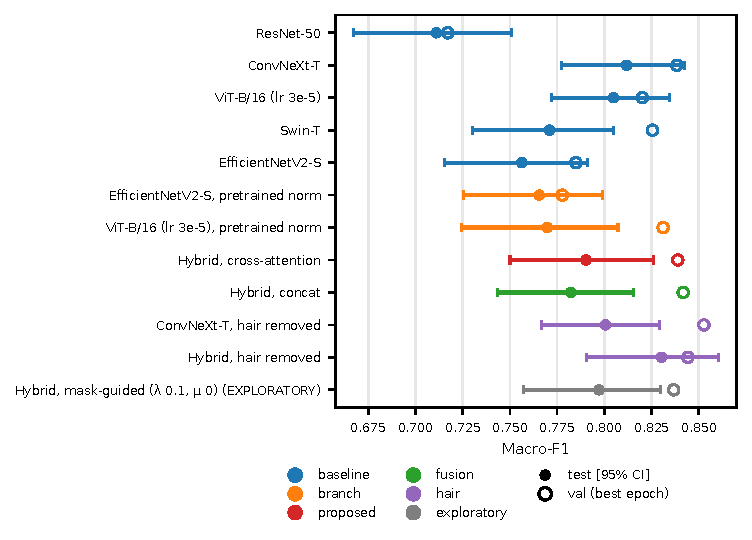
\includegraphics[width=\columnwidth]{figures/F1_ham10000_classification.pdf}
\caption{Test macro-F1 with 95\% CI (filled) and best-epoch validation macro-F1 (hollow) for every HAM10000 run,
coloured by role.}
\label{fig:f1}
\end{figure}

\begin{figure*}[!t]
\centering
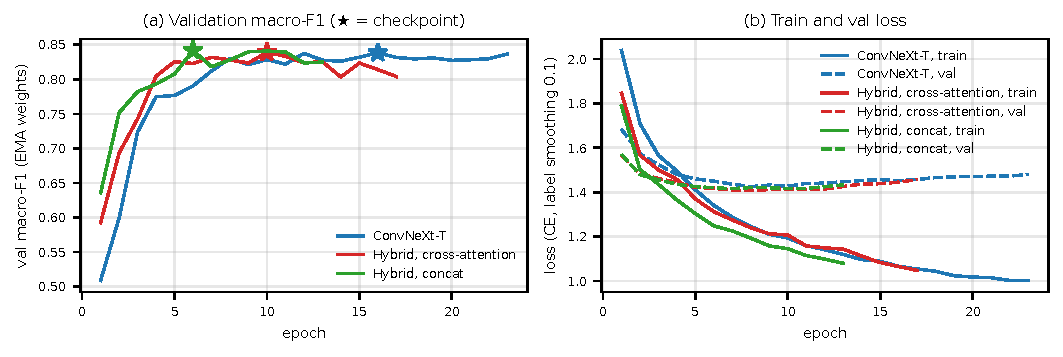
\includegraphics[width=\textwidth]{figures/F8_training_curves.pdf}
\caption{HAM10000 training history of ConvNeXt-T and both hybrids. (a) Validation macro-F1 with the checkpoint
epoch starred. (b) Training (solid) and validation (dashed) loss.}
\label{fig:train}
\end{figure*}

The hair-removed hybrid has the highest test macro-F1 of all runs (0.8302 [0.7906, 0.8603]) and the highest melanoma
sensitivity (0.726). This comparison was not planned in advance, and its validation score (0.8442) did not single
it out, so it is reported as an observation, not a finding.

\subsection{Paired Comparisons on HAM10000}
Overlapping confidence intervals are not a test, so the two pre-specified comparisons were tested with the paired
bootstrap (Table~\ref{tab:hampaired}, Fig.~\ref{fig:paired}). The hybrid's macro-F1 is 0.0215 lower than ConvNeXt-T's
(95\% CI $[-0.0542, 0.0069]$, Holm $p = 0.296$), and cross-attention is 0.0080 higher than concatenation
($[-0.0180, 0.0323]$, Holm $p = 0.480$). Neither difference is significant: the hybrid is not shown to beat the best
baseline, and cross-attention is not shown to beat concatenation.

\begin{table}[!t]
\centering
\caption{Paired Bootstrap on the HAM10000 Test Set (1,000 Shared Resamples; Holm over the Two Pre-Specified
Comparisons). \textsuperscript{\textdagger}Exploratory}
\label{tab:hampaired}
% Generated by scripts/make_report_tables.py; do not edit by hand.
% Sources: outputs/comparisons/ham10000_test_ham10000_hybrid_mask_l0.1_m0_vs_ham10000_hybrid.json, outputs/comparisons/ham10000_test_ham10000_hybrid_vs_ham10000_convnext_t.json, outputs/comparisons/ham10000_test_ham10000_hybrid_vs_ham10000_hybrid_concat.json
\small
\setlength{\tabcolsep}{3pt}
\renewcommand{\arraystretch}{1.1}
\begin{tabularx}{\columnwidth}{|>{\raggedright\arraybackslash}X|l|r|r|}
\hline
\textbf{$B-A$} & \textbf{$\Delta$ macro-F1 [95\% CI]} & \textbf{$p$} & \textbf{Holm $p$} \\ \hline
Hybrid $-$ ConvNeXt-T & \makecell[l]{$-0.0215$\\$[-0.0542, 0.0069]$} & $0.148$ & $0.296$ \\
Hybrid $-$ concat hybrid & \makecell[l]{$+0.0080$\\$[-0.0180, 0.0323]$} & $0.480$ & $0.480$ \\
Mask-guided $-$ hybrid\expl & \makecell[l]{$+0.0069$\\$[-0.0097, 0.0239]$} & $0.434$ & -- \\
\hline
\end{tabularx}

\end{table}

\begin{figure}[!t]
\centering
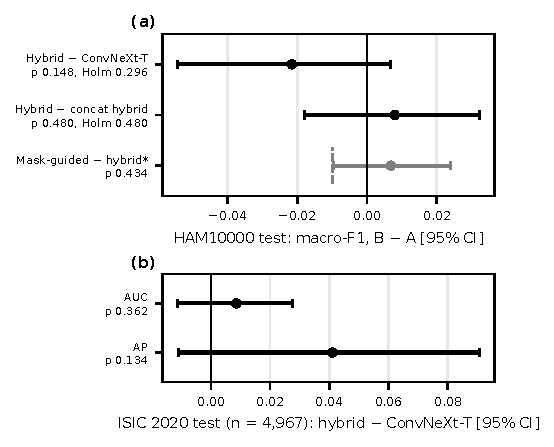
\includegraphics[width=\columnwidth]{figures/F2_paired_classification.pdf}
\caption{Paired differences: (a) HAM10000 macro-F1, (b) ISIC 2020 AUC and AP. The dashed line is the pre-set $-0.01$
``not worse'' margin of the exploratory mask-guided model (*).}
\label{fig:paired}
\end{figure}

Among the uncorrected secondary results, the hybrid's melanoma sensitivity is lower than ConvNeXt-T's (0.601 versus
0.679 in Table~\ref{tab:ham}; difference $-0.077$, $p = 0.042$, 101 versus 114 of 168 melanomas). With several
per-class tests, this is weak evidence, but it points in the clinically wrong direction.

\subsection{ISIC 2020 Melanoma Detection}
Table~\ref{tab:isic} and Fig.~\ref{fig:roc} show the ISIC 2020 test results. The hybrid's AUC (0.899) and AP (0.242)
are slightly higher than ConvNeXt-T's (0.891 and 0.201), but neither difference is significant
(Table~\ref{tab:isicpaired}: AUC $+0.009$ [$-0.011$, 0.028], $p = 0.362$; AP $+0.041$ [$-0.011$, 0.091],
$p = 0.134$).

\begin{table*}[!t]
\centering
\caption{ISIC 2020 Test (n = 4,967, 89 Melanoma). Cutoffs Fixed on Validation Before the Test Run. Images Tied
with a Cutoff Are Not Counted as Melanoma Here; the Paired Table Counts Them. Best AUC and AP in Bold}
\label{tab:isic}
% Generated by scripts/make_report_tables.py; do not edit by hand.
% Sources: outputs/runs/isic2020_convnext_t/eval/metrics.json, outputs/runs/isic2020_convnext_t/train_summary.json, outputs/runs/isic2020_effnetv2_s_pnorm/eval/metrics.json, outputs/runs/isic2020_effnetv2_s_pnorm/train_summary.json, outputs/runs/isic2020_hybrid/eval/metrics.json, outputs/runs/isic2020_hybrid/train_summary.json
\small
\setlength{\tabcolsep}{3pt}
\renewcommand{\arraystretch}{1.1}
\begin{tabular}{|l|r|r|l|l|c|c|c|}
\hline
\textbf{Model} & \textbf{Ep.} & \textbf{Val AUC} & \textbf{Test AUC [95\% CI]} & \textbf{AP [95\% CI]} & \multicolumn{3}{c|}{\textbf{Sens./spec. at cutoff}} \\
\cline{6-8}
 &  &  &  &  & \textbf{argmax} & \textbf{Youden} & \textbf{sens.\,$\geq$\,0.80} \\ \hline
ConvNeXt-T & 8 & $0.909$ & $0.891$ $[0.865, 0.916]$ & $0.201$ $[0.125, 0.296]$ & $0.213$/$0.988$ & $0.854$/$0.796$ & $0.809$/$0.826$ \\
Hybrid, cross-attention & 7 & {\boldmath $0.912$} & {\boldmath $0.899$} $[0.874, 0.923]$ & {\boldmath $0.242$} $[0.155, 0.336]$ & $0.213$/$0.991$ & $0.730$/$0.857$ & $0.730$/$0.868$ \\
EfficientNetV2-S, pretrained norm & 5 & $0.885$ & $0.895$ $[0.866, 0.922]$ & $0.218$ $[0.141, 0.321]$ & $0.225$/$0.991$ & $0.888$/$0.719$ & $0.809$/$0.795$ \\
\hline
\end{tabular}

\end{table*}

\begin{table*}[!t]
\centering
\caption{ISIC 2020 Paired Bootstrap (1,000 Shared Resamples): the Hybrid Minus ConvNeXt-T and Minus Its Local Branch
Alone (EfficientNetV2-S), Each Model at Its Own Validation Cutoffs}
\label{tab:isicpaired}
% Generated by scripts/make_report_tables.py; do not edit by hand.
% Sources: outputs/comparisons/isic2020_test_isic2020_hybrid_vs_isic2020_convnext_t.json, outputs/comparisons/isic2020_test_isic2020_hybrid_vs_isic2020_effnetv2_s_pnorm.json
\small
\setlength{\tabcolsep}{3pt}
\renewcommand{\arraystretch}{1.1}
\begin{tabular}{|l|r|r|r|l|r|r|r|l|r|}
\hline
 &  & \multicolumn{4}{c|}{\textbf{Hybrid $-$ ConvNeXt-T}} & \multicolumn{4}{c|}{\textbf{Hybrid $-$ EfficientNetV2-S}} \\
\cline{3-10}
\textbf{Metric} & \textbf{Hybrid} & \textbf{ConvNeXt-T} & \textbf{$\Delta$} & \textbf{[95\% CI]} & \textbf{$p$} & \textbf{EffNetV2-S} & \textbf{$\Delta$} & \textbf{[95\% CI]} & \textbf{$p$} \\ \hline
AUC & $0.899$ & $0.891$ & $+0.009$ & $[-0.011, 0.028]$ & $0.362$ & $0.895$ & $+0.004$ & $[-0.013, 0.022]$ & $0.662$ \\
AP & $0.242$ & $0.201$ & $+0.041$ & $[-0.011, 0.091]$ & $0.134$ & $0.218$ & $+0.024$ & $[-0.022, 0.064]$ & $0.390$ \\
Spec. @ sens.\,$\geq$\,0.80 & $0.868$ & $0.826$ & $+0.042$ & $[0.034, 0.051]$ & $<0.002$ & $0.795$ & $+0.073$ & $[0.063, 0.083]$ & $<0.002$ \\
Sens. @ sens.\,$\geq$\,0.80 & $0.730$ & $0.809$ & $-0.079$ & $[-0.184, 0.031]$ & $0.214$ & $0.809$ & $-0.079$ & $[-0.151, -0.011]$ & $0.040$ \\
Spec. @ Youden & $0.857$ & $0.796$ & $+0.062$ & $[0.052, 0.072]$ & $<0.002$ & $0.718$ & $+0.139$ & $[0.128, 0.151]$ & $<0.002$ \\
Sens. @ Youden & $0.730$ & $0.854$ & $-0.124$ & $[-0.219, -0.024]$ & $0.016$ & $0.888$ & $-0.157$ & $[-0.244, -0.082]$ & $<0.002$ \\
Spec. @ argmax & $0.991$ & $0.988$ & $+0.003$ & $[0.000, 0.006]$ & $0.068$ & $0.991$ & $+0.000$ & $[-0.003, 0.002]$ & $1.000$ \\
Sens. @ argmax & $0.213$ & $0.213$ & $+0.000$ & $[-0.074, 0.075]$ & $1.000$ & $0.225$ & $-0.011$ & $[-0.078, 0.060]$ & $0.908$ \\
\hline
\end{tabular}

\end{table*}

\begin{figure*}[!t]
\centering
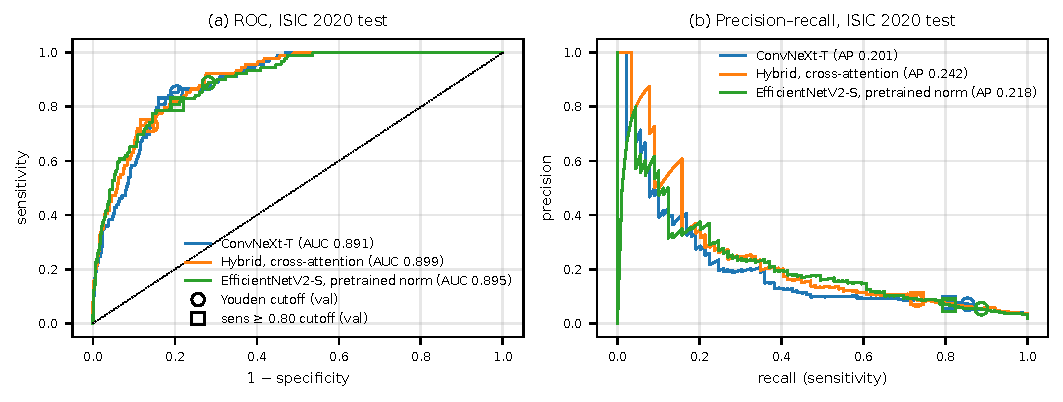
\includegraphics[width=\textwidth]{figures/F3_isic2020_roc_pr.pdf}
\caption{(a) ROC and (b) precision--recall curves on the ISIC 2020 test set. Circles mark the Youden cutoff
and squares the sensitivity $\geq 0.80$ cutoff, both fixed on validation.}
\label{fig:roc}
\end{figure*}

At the cutoffs fixed on validation, the two models land at different operating points. The hybrid's cutoff for
sensitivity $\geq 0.80$ did not transfer to the test set: it catches 0.730 of melanomas, against 0.809 for
ConvNeXt-T. Its higher specificity at that cutoff ($+0.042$) and at the Youden cutoff ($+0.062$) is therefore paid
for with lower sensitivity (Youden: $-0.124$ [$-0.219$, $-0.024$], $p = 0.016$). Neither model is shown to be better
at equal sensitivity.

The local branch alone (EfficientNetV2-S with pretrained normalisation) is the third ISIC 2020 model; it isolates
what the Swin branch and the fusion add. Its test AUC is 0.895 [0.866, 0.922] and its AP 0.218 [0.141, 0.321],
between ConvNeXt-T and the hybrid, although its validation AUC was the lowest of the three (0.885 against 0.909 and
0.912). The hybrid is not significantly better than its own local branch (Table~\ref{tab:isicpaired}: AUC $+0.004$
[$-0.013$, 0.022], $p = 0.662$; AP $+0.024$ [$-0.022$, 0.064], $p = 0.390$). Like ConvNeXt-T's, the local branch's
sensitivity cutoff transferred to the test set (0.809), so at the fixed cutoffs the hybrid again trades sensitivity
for specificity (at the sensitivity $\geq 0.80$ cutoff: specificity $+0.073$, sensitivity $-0.079$ [$-0.151$,
$-0.011$], $p = 0.040$).

\subsection{Localisation Against Lesion Masks}
Table~\ref{tab:loc} and Fig.~\ref{fig:loc} report how well the maps match the lesion masks on the HAM10000
validation set. Lesions are large: they cover 41.8\% of the image crop on average, so a uniform map already scores
IoU 0.418 and a centred Gaussian 0.487. Against these references most maps localise poorly. Only ResNet-50 (0.533),
the ViT-B/16 with pretrained normalisation (0.496) and the hybrid's local map (0.490) exceed the centred Gaussian;
ConvNeXt-T scores 0.311.

\begin{table}[!t]
\centering
\caption{Localisation on HAM10000 Validation (n = 1,503), Grad-CAM for the Predicted Class Unless Named. Rand.:
Same Architecture with Random Weights. Best Trained Map per Column in Bold}
\label{tab:loc}
% Generated by scripts/make_report_tables.py; do not edit by hand.
% Sources: outputs/runs/ham10000_convnext_t/xai_val/summary.json, outputs/runs/ham10000_convnext_t/xai_val_random/summary.json, outputs/runs/ham10000_convnext_t_hair/xai_val/summary.json, outputs/runs/ham10000_convnext_t_hair/xai_val_random/summary.json, outputs/runs/ham10000_effnetv2_s/xai_val/summary.json, outputs/runs/ham10000_effnetv2_s/xai_val_random/summary.json, outputs/runs/ham10000_effnetv2_s_pnorm/xai_val/summary.json, outputs/runs/ham10000_effnetv2_s_pnorm/xai_val_random/summary.json, outputs/runs/ham10000_hybrid/xai_val/summary.json, outputs/runs/ham10000_hybrid/xai_val_random/summary.json, outputs/runs/ham10000_hybrid_concat/xai_val/summary.json, outputs/runs/ham10000_hybrid_concat/xai_val_random/summary.json, outputs/runs/ham10000_hybrid_hair/xai_val/summary.json, outputs/runs/ham10000_hybrid_hair/xai_val_random/summary.json, outputs/runs/ham10000_resnet50/xai_val/summary.json, outputs/runs/ham10000_resnet50/xai_val_random/summary.json, outputs/runs/ham10000_swin_t/xai_val/summary.json, outputs/runs/ham10000_swin_t/xai_val_random/summary.json, outputs/runs/ham10000_vit_b16_lr3e-5/xai_val/summary.json, outputs/runs/ham10000_vit_b16_lr3e-5/xai_val_random/summary.json, outputs/runs/ham10000_vit_b16_pnorm_lr3e-5/xai_val/summary.json, outputs/runs/ham10000_vit_b16_pnorm_lr3e-5/xai_val_random/summary.json
\small
\setlength{\tabcolsep}{3pt}
\renewcommand{\arraystretch}{1.1}
\begin{tabularx}{\columnwidth}{|>{\raggedright\arraybackslash}X|r|r|r|r|}
\hline
\textbf{Model / map} & \textbf{IoU} & \textbf{Point.} & \textbf{Energy} & \textbf{Rand. IoU} \\ \hline
ResNet-50 & {\boldmath $0.533$} & $0.968$ & {\boldmath $0.711$} & $0.418$ \\
ConvNeXt-T & $0.311$ & $0.910$ & $0.521$ & $0.246$ \\
Swin-T & $0.453$ & $0.504$ & $0.530$ & $0.336$ \\
EfficientNetV2-S, pretrained norm & $0.446$ & $0.870$ & $0.570$ & $0.373$ \\
ViT-B/16 (lr 3e-5), pretrained norm & $0.496$ & {\boldmath $0.974$} & $0.644$ & $0.060$ \\
Hybrid: Grad-CAM, EffNetV2 branch & $0.490$ & $0.884$ & $0.706$ & $0.223$ \\
Hybrid: Grad-CAM, Swin branch & $0.410$ & $0.611$ & $0.468$ & $0.285$ \\
Hybrid: Grad-CAM, fused & $0.422$ & $0.849$ & $0.446$ & $0.418$ \\
Hybrid: cross-attn, EffNetV2 $\rightarrow$ Swin & $0.277$ & $0.866$ & $0.557$ & $0.418$ \\
Hybrid: cross-attn, Swin $\rightarrow$ EffNetV2 & $0.228$ & $0.967$ & $0.655$ & $0.418$ \\
\hline
\textit{Reference: centred Gaussian} & $0.487$ & $0.961$ & $0.603$ & -- \\
\textit{Reference: uniform map} & $0.418$ & -- & $0.418$ & -- \\
\hline
\end{tabularx}

\end{table}

\begin{figure*}[p]
\centering
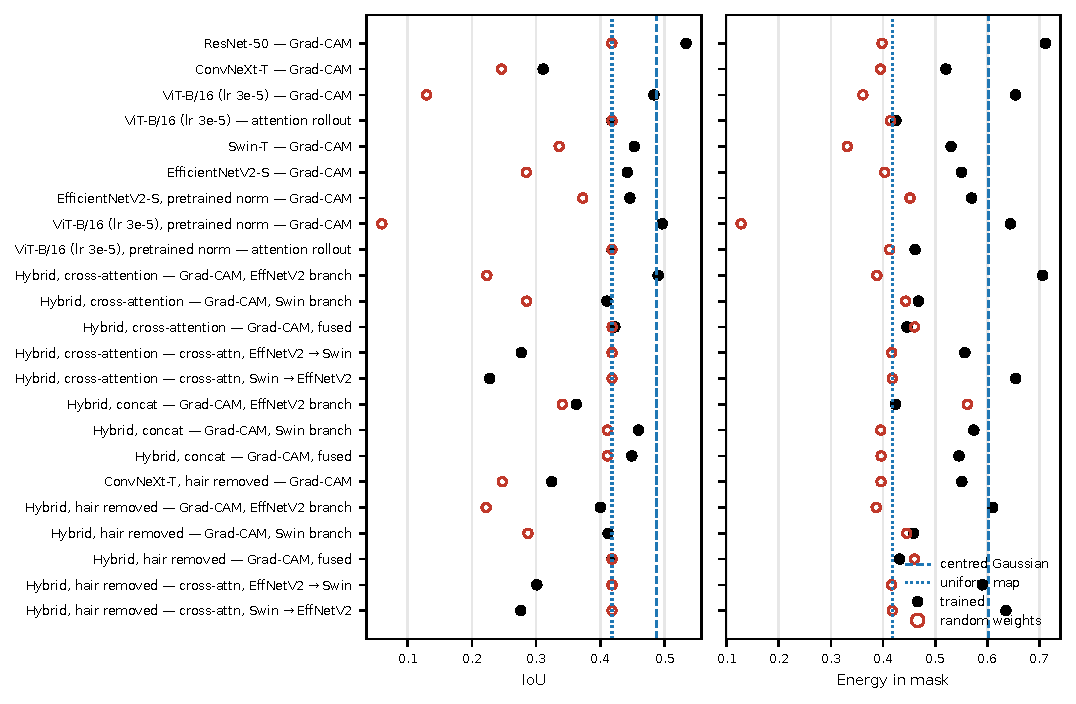
\includegraphics[width=\textwidth]{figures/F4_ham10000_localisation_val.pdf}
\caption{IoU (left) and energy in the lesion mask (right) for every map on HAM10000 validation, trained (filled)
and with random weights (hollow), against a centred Gaussian (dashed) and a uniform map (dotted).}
\label{fig:loc}
\end{figure*}

The hybrid's fused map scores about the uniform map's IoU (0.422 versus 0.418), and exactly 0.418 with random
weights: it is flat enough that the 15\% threshold keeps almost the whole image. The cross-attention maps point at
the lesion (pointing 0.866 and 0.967) but cover a small area (IoU 0.277 and 0.228).

\subsection{Explanation Trust (Confirmatory)}
Table~\ref{tab:trust} gives the confirmatory test. The decision rule, Eq.~(\ref{eq:rule}), is not met for either
hybrid map.

\begin{table*}[!t]
\centering
\caption{Explanation Trust on the HAM10000 Test Set (Confirmatory, n = 1,503): Hybrid Map ($B$) Minus ConvNeXt-T
Grad-CAM ($A$). $\downarrow$/$\uparrow$: Lower / Higher Is Better. \better/\worse: Significantly Better / Worse for
$B$ (Holm over 12 Tests; $<0.024$: No Resample Crossed Zero)}
\label{tab:trust}
% Generated by scripts/make_report_tables.py; do not edit by hand.
% Sources: outputs/comparisons/ham10000_xai_test_ham10000_hybrid_vs_ham10000_convnext_t.json
\small
\setlength{\tabcolsep}{3pt}
\renewcommand{\arraystretch}{1.1}
\begin{tabularx}{\textwidth}{|>{\raggedright\arraybackslash}X|r|r|l|l|r|l|l|}
\hline
 &  & \multicolumn{3}{c|}{\textbf{Hybrid, local map}} & \multicolumn{3}{c|}{\textbf{Hybrid, fused map}} \\
\cline{3-8}
\textbf{Endpoint} & \textbf{ConvNeXt-T} & \textbf{Hybrid} & \textbf{$B-A$ [95\% CI]} & \textbf{Holm $p$} & \textbf{Hybrid} & \textbf{$B-A$ [95\% CI]} & \textbf{Holm $p$} \\ \hline
Deletion $-$ random $\downarrow$ & $-0.078$ & $-0.028$ & \worse$+0.051$ $[0.041, 0.061]$ & $<0.024$ & $-0.075$ & $+0.003$ $[-0.007, 0.012]$ & $0.640$ \\
Insertion $-$ random $\uparrow$ & $0.058$ & $0.032$ & \worse$-0.027$ $[-0.034, -0.020]$ & $<0.024$ & $0.048$ & \worse$-0.011$ $[-0.017, -0.004]$ & $0.008$ \\
SSIM to randomised $\downarrow$ & $0.268$ & $0.262$ & $-0.006$ $[-0.015, 0.002]$ & $0.360$ & $0.292$ & \worse$+0.023$ $[0.011, 0.035]$ & $<0.024$ \\
Stability ($\rho$) $\uparrow$ & $0.938$ & $0.707$ & \worse$-0.232$ $[-0.246, -0.218]$ & $<0.024$ & $0.892$ & \worse$-0.047$ $[-0.053, -0.041]$ & $<0.024$ \\
IoU $\uparrow$ & $0.315$ & $0.499$ & \better$+0.184$ $[0.169, 0.199]$ & $<0.024$ & $0.437$ & \better$+0.122$ $[0.110, 0.133]$ & $<0.024$ \\
IoU gap (correct $-$ wrong) $\uparrow$ & $-0.031$ & $0.084$ & \better$+0.115$ $[0.076, 0.156]$ & $<0.024$ & $-0.071$ & $-0.040$ $[-0.080, 0.002]$ & $0.204$ \\
\hline
\textit{Frozen decision rule} &  & \multicolumn{3}{c|}{not met} & \multicolumn{3}{c|}{not met} \\
\hline
\end{tabularx}

\end{table*}

The local map is significantly \textit{less} faithful than ConvNeXt-T's map on both deletion ($+0.051$) and
insertion ($-0.027$), shows no difference after randomisation (Holm $p = 0.360$), and is much less stable (Spearman
0.707 versus 0.938). The fused map does not differ on deletion (Holm $p = 0.640$) but is worse on insertion
(Holm $p = 0.008$), more similar to its randomised version (SSIM $+0.023$), and less stable (0.892 versus 0.938).

Where the hybrid is better is localisation. IoU is higher for both maps ($+0.184$ local, $+0.122$ fused), and the
local map localises worse when the model is wrong (IoU gap 0.084 against $-0.031$ for ConvNeXt-T; difference $+0.115$),
which is how a trustworthy explanation should behave. Every primary endpoint has the same direction as on
validation.

Fig.~\ref{fig:trust} shows why. ConvNeXt-T's insertion curve rises steeply: restoring the few pixels its map ranks
highest already brings back most of the class probability. The hybrid's curves lie closer to its random-map
reference than ConvNeXt-T's do. Fig.~\ref{fig:qual} shows the maps on one fixed-seed test image per class: ConvNeXt-T highlights small, peaked
regions, the hybrid's local map covers more of the lesion, and the fused map covers most of the image.

\begin{figure*}[!t]
\centering
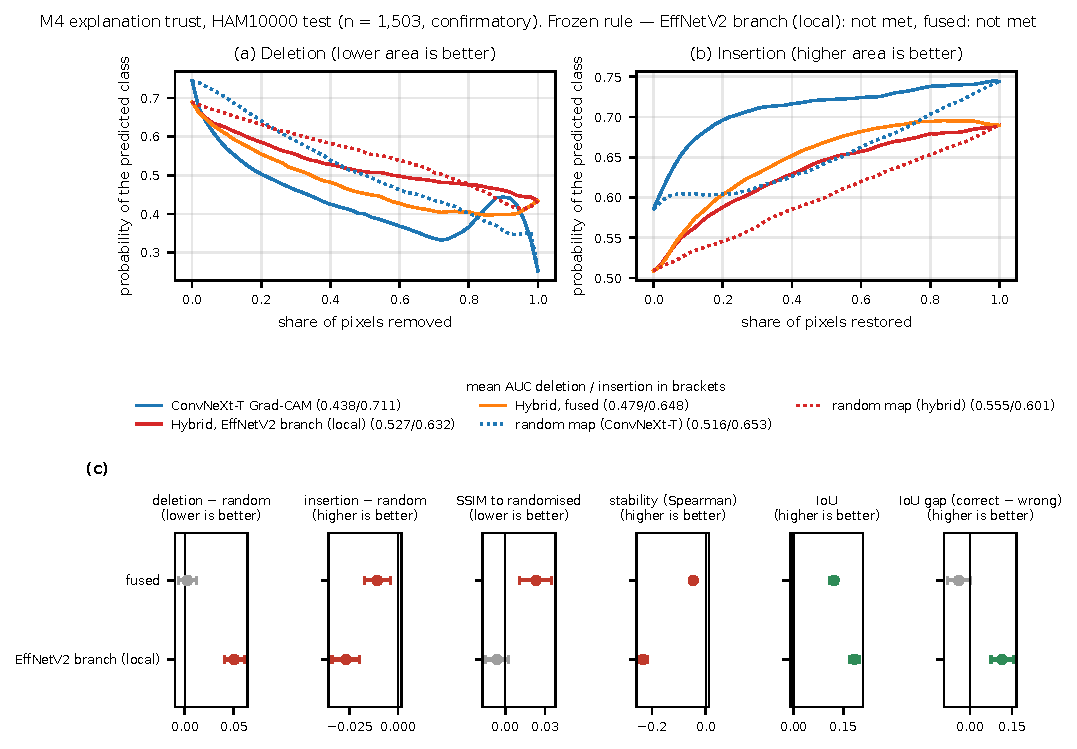
\includegraphics[width=\textwidth]{figures/F5_m4_trust_test.pdf}
\caption{Explanation trust on the HAM10000 test set. (a) Mean deletion and (b) insertion curves; the legend gives each
map's mean deletion / insertion AUC, including each model's random-map reference. (c) Paired differences on the six primary endpoints
(green / red: significantly better / worse for the hybrid map after Holm correction; grey: not significant).}
\label{fig:trust}
\end{figure*}

\begin{figure*}[p]
\centering
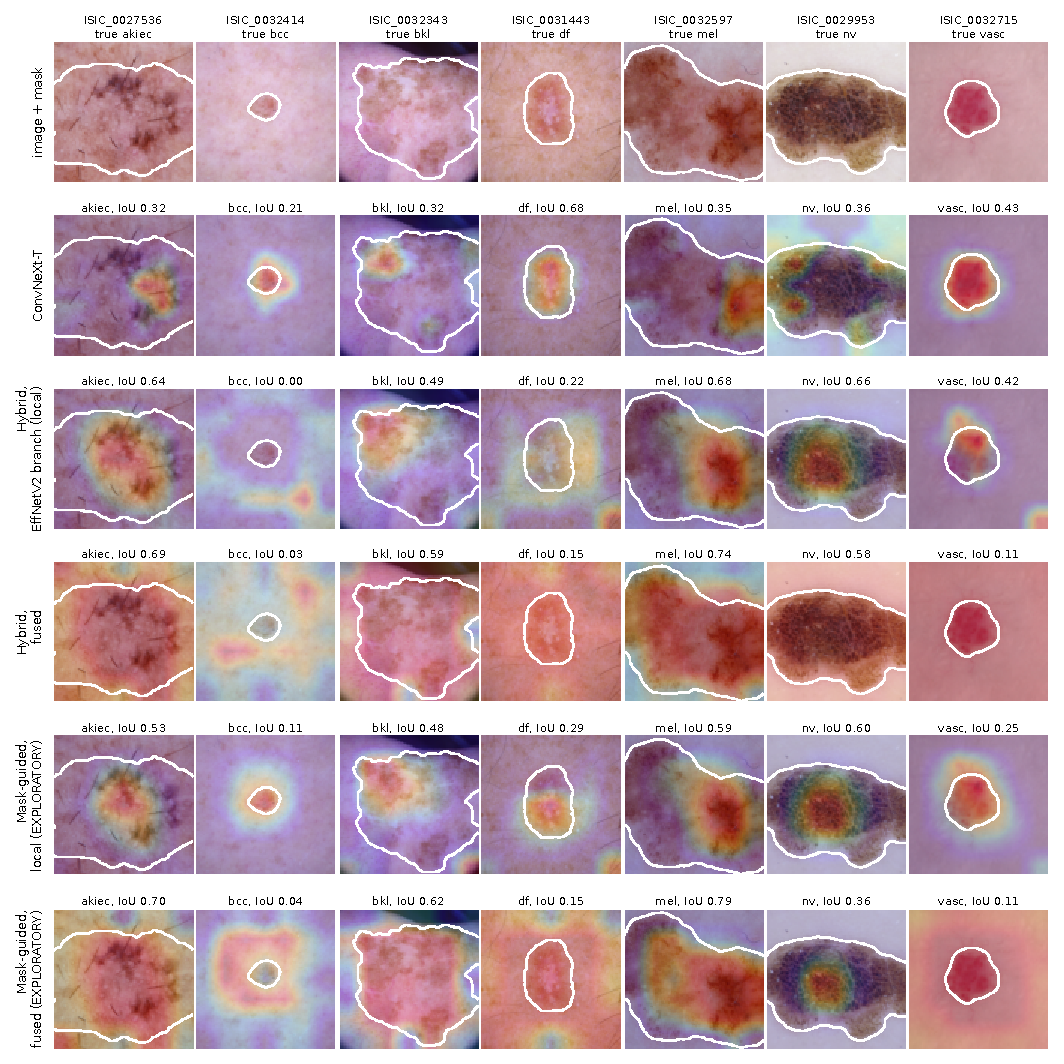
\includegraphics[width=\textwidth]{figures/F6_qualitative_test.pdf}
\caption{Grad-CAM for the predicted class on HAM10000 test images (white: lesion mask). Images are the first of two
per class drawn with a fixed seed, not selected by eye. Panel titles: predicted class (\texttimes{} = wrong) and IoU.
The mask-guided rows are exploratory.}
\label{fig:qual}
\end{figure*}

\subsection{Parameter Randomisation Examples}
Fig.~\ref{fig:rand} illustrates the randomisation check on the same images. After all blocks are re-initialised,
the maps of all three kinds change visibly, as the check requires; some of the hybrid's fused maps become entirely
zero, because the ReLU in Eq.~(\ref{eq:fused}) removes every value. These examples use
a different random draw from the confirmatory test, whose scores (Table~\ref{tab:trust}) remain the reported ones.

\begin{figure*}[p]
\centering
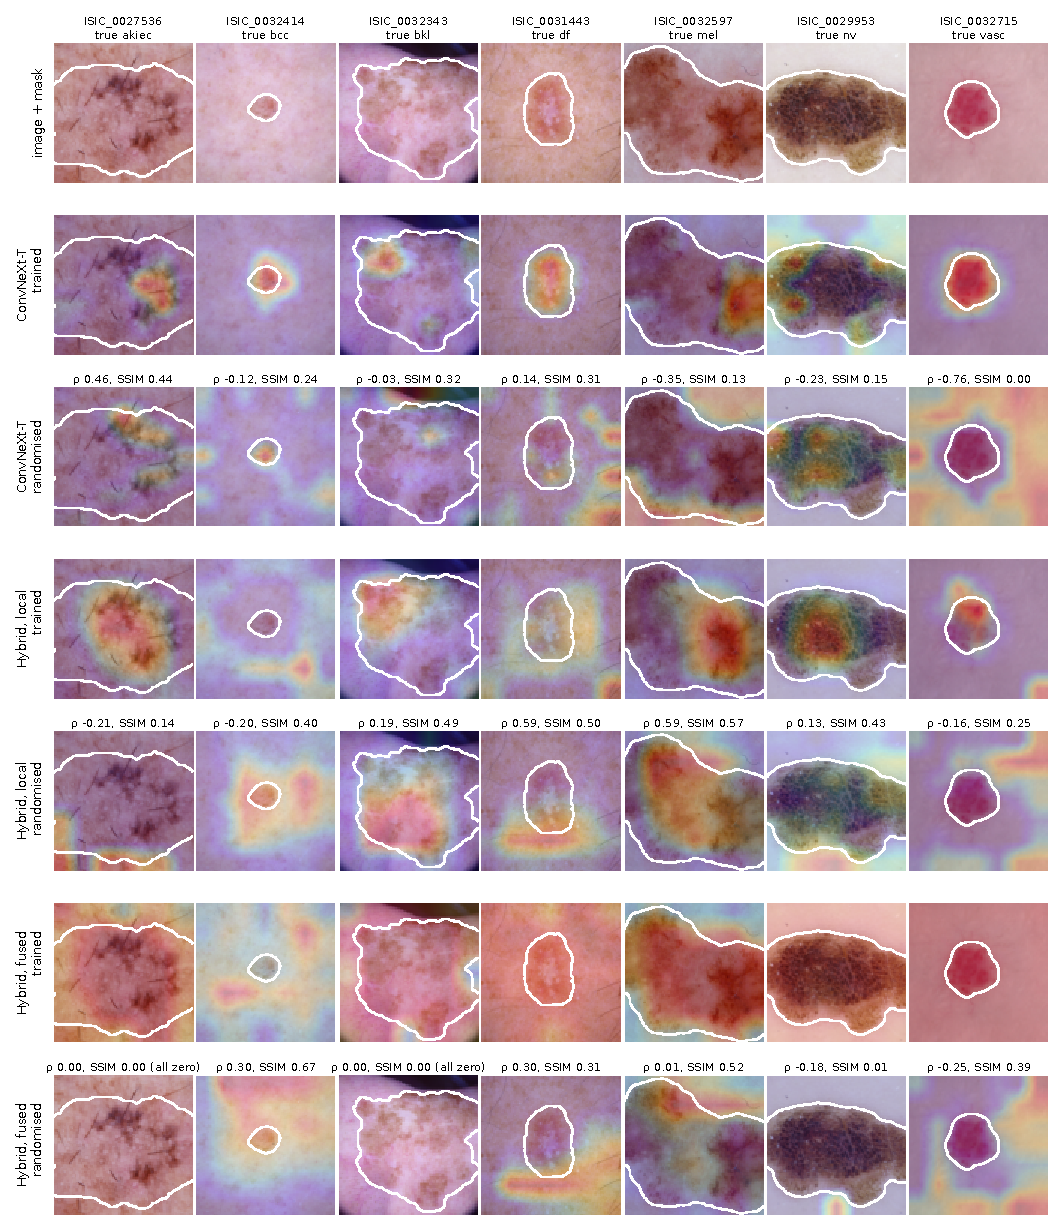
\includegraphics[width=\textwidth]{figures/F9_randomisation_test.pdf}
\caption{Grad-CAM before and after re-initialising every block of the model, with the rank correlation ($\rho$) and
SSIM between the two maps (an all-zero map is shown without overlay). Same images as Fig.~\ref{fig:qual}.}
\label{fig:rand}
\end{figure*}

\subsection{Exploratory Follow-ups}
Fig.~\ref{fig:partb} summarises the three follow-ups on validation and test. All results in this subsection are
exploratory.

\begin{figure*}[!t]
\centering
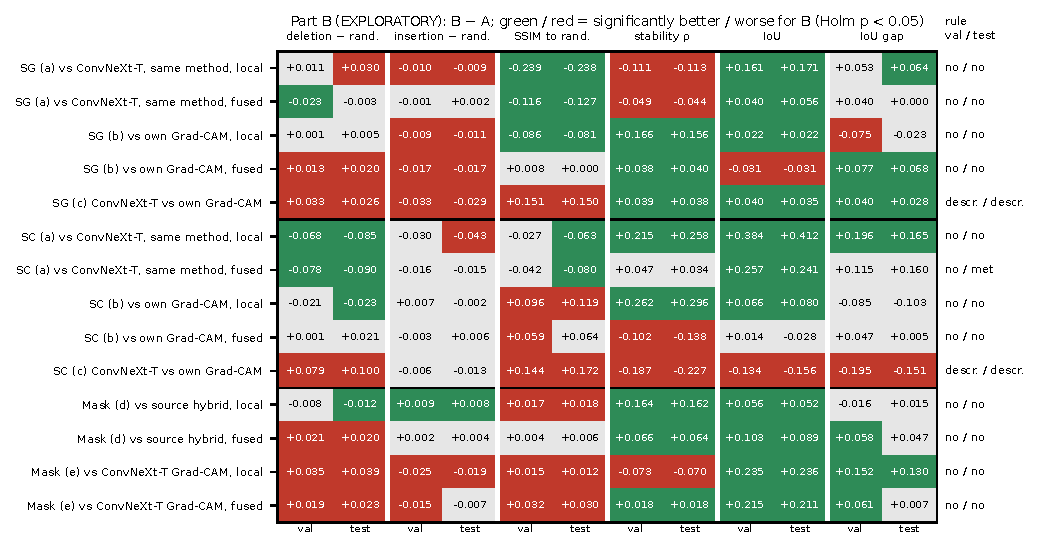
\includegraphics[width=\textwidth]{figures/F7_part_b_summary.pdf}
\caption{Exploratory follow-ups: $B-A$ on the primary endpoints, validation and test. SG: SmoothGrad-CAM; SC:
Score-CAM; Mask: mask-guided fine-tuning. Comparisons (a) hybrid versus ConvNeXt-T with the same method, (b) method
versus the hybrid's own Grad-CAM, (c) method versus ConvNeXt-T's own Grad-CAM (descriptive), (d) mask-guided versus
the original hybrid, (e) mask-guided versus ConvNeXt-T Grad-CAM.}
\label{fig:partb}
\end{figure*}

\subsubsection{SmoothGrad-CAM}
SmoothGrad-CAM meets the rule in none of the four comparisons on validation or test. On the hybrid's local map it
raises stability ($+0.156$ on test) and lowers the similarity to the randomised map ($-0.081$), but it lowers
faithfulness on insertion. Its apparent advantage over ConvNeXt-T on randomisation comes largely from ConvNeXt-T
getting worse: SmoothGrad raises ConvNeXt-T's randomisation SSIM by $+0.150$ on test.

\subsubsection{Score-CAM}
Score-CAM formally meets the rule once, on test, for the fused map against ConvNeXt-T (deletion $-0.090$,
randomisation SSIM $-0.080$). This is not evidence of a more trustworthy map. On ConvNeXt-T, 27 of 150 validation and
24 of 150 test Score-CAM maps are entirely zero: its last stage has signed activations (about 51\% negative), the
Score-CAM weights are all positive and nearly equal, and the weighted sum is negative wherever the channel mean is.
On the hybrid's local map, Score-CAM is worse than Grad-CAM after randomisation in both splits.

\subsubsection{Mask-Guided Fine-Tuning}
Only one of the five candidates kept its validation macro-F1 within 0.01 of the original model
(Table~\ref{tab:selection}); the others lost between 0.013 and 0.029. The chosen model ($\lambda = 0.1$, $\mu = 0$)
moves its maps onto the lesion: on test, the fused map's IoU rises from 0.437 to 0.526 and its energy in the mask
from 0.459 to 0.801, and both maps become more stable ($+0.162$ local, $+0.064$ fused). Its local map becomes more
faithful than the original's on deletion ($-0.012$) and insertion ($+0.008$), but more similar to its randomised
version ($+0.018$), so the rule is still not met; against ConvNeXt-T it remains less faithful. Classification is
not worse by the pre-set criterion: macro-F1 $+0.0069$ [$-0.0097$, 0.0239], whose lower bound lies just inside the
$-0.01$ margin.

\begin{table}[!t]
\centering
\caption{Mask-Guided Fine-Tuning: Candidates and Selection on Validation (Exploratory). Eligible: Validation
Macro-F1 Within 0.01 of the Source; Screening on a Fixed 300-Image Validation Subset, Fused Map}
\label{tab:selection}
% Generated by scripts/make_report_tables.py; do not edit by hand.
% Sources: outputs/comparisons/ham10000_mask_guided_consistency.json, outputs/comparisons/ham10000_mask_guided_lambda.json
\small
\setlength{\tabcolsep}{3pt}
\renewcommand{\arraystretch}{1.1}
\begin{tabularx}{\columnwidth}{|>{\raggedright\arraybackslash}X|r|r|r|c|r|r|c|}
\hline
\textbf{Stage} & \textbf{$\lambda$} & \textbf{$\mu$} & \textbf{Val F1} & \textbf{Elig.} & \textbf{Ins.\,$-$\,rand.} & \textbf{IoU} & \textbf{Chosen} \\ \hline
source & -- & -- & $0.8389$ & -- & $0.047$ & $0.410$ &  \\
1 ($\lambda$) & $0.1$ & $0$ & $0.8367$ & yes & $0.049$ & $0.518$ & $\checkmark$ \\
1 ($\lambda$) & $0.3$ & $0$ & $0.8257$ & no & $0.045$ & $0.196$ &  \\
1 ($\lambda$) & $1$ & $0$ & $0.8166$ & no & $0.041$ & $0.263$ &  \\
2 ($\mu$) & $0.1$ & $0.1$ & $0.8102$ & no & $0.059$ & $0.559$ &  \\
2 ($\mu$) & $0.1$ & $1$ & $0.8143$ & no & $0.036$ & $0.406$ &  \\
\hline
\end{tabularx}

\end{table}

% =================================================================================================== 5
\section{Discussion}

\subsection{Fusion Did Not Improve Classification}
On HAM10000 the hybrid is above both of its branches trained alone, so combining local and global features helps
relative to either branch there; on ISIC 2020, however, it is not significantly better than its local branch
(AUC $+0.004$, $p = 0.662$). It does not, however, beat a single modern CNN: ConvNeXt-T is 0.0215 macro-F1 ahead on test, and
cross-attention adds nothing measurable over concatenation. With about 7,000 training images, a well-tuned
ConvNeXt-T already captures the information that the second branch adds. The hybrid also dropped more from
validation to test than ConvNeXt-T did, which suggests that its larger capacity (55.61 million parameters) fits the
validation set more closely.

\subsection{Localisation Is Not Faithfulness}
The central result is a dissociation. The hybrid's local map overlaps the lesion better than any ConvNeXt-T map, yet
removing or restoring the pixels it ranks highest changes the prediction less than for ConvNeXt-T. A map can cover the
lesion because lesion pixels share texture that the local branch responds to, without those pixels being the ones
that drive the decision after fusion; this explanation is a hypothesis that the present experiments do not test.
ConvNeXt-T's small, peaked maps localise poorly by IoU but point at regions
whose removal changes the output. Evaluating explanations by IoU alone would have reached the opposite conclusion.

\subsection{Sanity Checks and Flat Maps}
The randomisation test depends on the similarity measure. By the pre-registered SSIM, the fused map is worse than
ConvNeXt-T's; by absolute rank correlation (exploratory), both hybrid maps change more than ConvNeXt-T's. Flat
maps score a high SSIM against almost anything, and the fused map is flat (its IoU equals the uniform map's).
Reporting several similarity measures, as done here, makes this disagreement visible instead of hiding it.

\subsection{What the Exploratory Follow-ups Show}
Changing the explanation method did not help. SmoothGrad-CAM trades faithfulness for stability, and Score-CAM fails
outright on a layer with signed activations, which is a property of the layer rather than a flaw of the method's
formula. Mask-guided fine-tuning changes where the maps point, not what the model uses: localisation and stability
improve while faithfulness against ConvNeXt-T does not.

\subsection{What We Achieved and What We Did Not}
\textbf{What worked:}
\begin{itemize}
\item \textit{Leakage-free evaluation:} lesion-grouped splits (5,230 / 1,122 / 1,118 lesions in
Table~\ref{tab:splits}) and patient-grouped ISIC 2020 splits, with each test set used once per model.
\item \textit{A pre-registered protocol:} endpoints and decision rule were fixed on validation; the four changes made
there are documented, and nothing was changed after the test run.
\item \textit{Better localisation:} the hybrid's local map has a higher test IoU than ConvNeXt-T's (0.499 versus
0.315, $+0.184$, Holm $p < 0.024$), as does the fused map ($+0.122$).
\item \textit{An explanation that degrades when the model is wrong:} the local map's IoU gap is $+0.115$
[0.076, 0.156] higher than ConvNeXt-T's, consistent on validation and test.
\item \textit{Mask-guided gains (exploratory):} fused-map IoU 0.437 $\rightarrow$ 0.526, stability $+0.162$ (local)
and $+0.064$ (fused), and local-map faithfulness better than the original hybrid's, with classification not worse
(lower CI bound $-0.0097$).
\item \textit{The hybrid beats its own branches} on HAM10000 test macro-F1 (0.7903 versus 0.7655 and 0.7710; not
tested pairwise).
\end{itemize}
\textbf{What did not work:}
\begin{itemize}
\item \textit{Classification:} the hybrid is not better than ConvNeXt-T (macro-F1 0.7903 versus 0.8118, $-0.0215$,
Holm $p = 0.296$) and cross-attention is not better than concatenation ($+0.0080$, Holm $p = 0.480$); its melanoma
sensitivity is lower (0.601 versus 0.679, uncorrected $p = 0.042$).
\item \textit{ISIC 2020:} no significant gain over ConvNeXt-T in AUC ($+0.009$, $p = 0.362$) or AP ($+0.041$,
$p = 0.134$), nor over the local branch alone (AUC $+0.004$, $p = 0.662$), and the hybrid's sensitivity cutoff did
not transfer (0.730 on test, against 0.809 for both other models).
\item \textit{Explanation trust:} the decision rule is not met for either hybrid map. The local map is less faithful
(deletion $+0.051$, insertion $-0.027$) and less stable ($-0.232$); the fused map is worse on insertion
(Holm $p = 0.008$), randomisation SSIM ($+0.023$) and stability ($-0.047$).
\item \textit{Exploratory methods:} SmoothGrad-CAM meets the rule in 0 of 8 checks and mask-guided fine-tuning in 0 of 8
(validation and test); Score-CAM's single formal pass is caused by 24 of 150 all-zero ConvNeXt-T maps on test.
\item \textit{Generalisation gap:} the hybrid lost 0.0486 macro-F1 from validation to test (0.8389 to 0.7903).
\end{itemize}

% =================================================================================================== 6
\section{Limitations}

\subsection{Statistical Design}
Every model was trained once with one seed, so the confidence intervals cover variation over test images, not over
training runs; validation differences of about 0.01 macro-F1 are within run-to-run noise. The HAM10000 test set was
used by the confirmatory explanation test, then by the classification test of the remaining runs, then by the
exploratory follow-ups, which is why everything after the confirmatory test is labelled exploratory. The rare
classes are too small for per-class conclusions (17 \textit{df} and 21 \textit{vasc} test images).

\subsection{Data}
The ISIC 2020 images are a resized $256\times256$ copy in which non-square images are stretched, only the public
training set is used, and there are no lesion masks. ResNet-50, ViT-B/16 and Swin-T were not trained on ISIC 2020
because of the GPU quota. HAM10000 comes from two sites and records no skin type, so behaviour on other skin types
and devices is untested. Lesions cover 41.8\% of the crop on average, which makes IoU easy to match with a diffuse
map. DullRazor sometimes removes lesion borders, the region the IoU is measured on.

\subsection{Explanation Metrics}
Deletion and insertion create inputs unlike the training images, so part of each score reflects the model's response
to such inputs; the random-map baseline reduces but does not remove this. Each randomisation test uses one random
draw. The stability test uses four perturbations, and the noise perturbation changes the prediction for 17.6\%
(ConvNeXt-T) and 19.5\% (hybrid) of test images, which are then excluded for that perturbation. Score-CAM ran on 150
images per split, and no clinician has rated any map.

\subsection{Numerical Precision and Compute}
With mixed precision, predicted probabilities are quantised, and test images tied with a cutoff change the
specificity slightly depending on the comparison precision: 0.8264 or 0.8255 for ConvNeXt-T at one cutoff (four
images), and 0.7187 or 0.7181 and 0.7952 or 0.7946 for EfficientNetV2-S at its two cutoffs (three images each). The
fixed rule was not changed after the test runs. All HAM10000 models were trained on a 4 GB GPU with gradient checkpointing and
accumulation.

% =================================================================================================== 7
\section{Future Work}
Several directions follow from the results:
\begin{itemize}
\item \textbf{Mask-guided training at scale:} use the segmented images of the ISIC 2018 lesion
segmentation task as a second mask source, train with at least three seeds, and supervise the local
branch as well, which needs second-order gradients and a larger GPU.
\item \textbf{External testing on PH2:} its dermoscopic images with lesion masks, used for
segmentation by WA-NET \cite{hu2025wanet}, allow a melanoma-versus-nevus and localisation test on unseen data.
\item \textbf{Clinical criteria with Derm7pt:} test whether the highlighted features carry the seven-point checklist
criteria annotated in the Derm7pt dataset, for example with concept-based probes, since its labels are per image
rather than per region.
\item \textbf{Domain shift with ISIC 2024:} evaluate on the ISIC 2024 lesion crops from total-body photographs,
which are not dermoscopic, first without and then with fine-tuning.
\item \textbf{Self-supervised pretraining:} pretrain both branches on unlabelled dermoscopy with contrastive or
self-distillation methods and repeat the trust protocol.
\item \textbf{Clinician review:} a blinded rating of the maps by dermatologists, with a rating protocol written in
advance and inter-rater agreement reported.
\item \textbf{Remaining baselines:} train ResNet-50, ViT-B/16 and Swin-T on ISIC 2020, and evaluate Score-CAM on
a layer with non-negative activations.
\end{itemize}

% =================================================================================================== 8
\section{Conclusion}
This work built a hybrid CNN--Transformer for dermoscopic lesion classification, with an EfficientNetV2-S local
branch, a Swin-T global branch and bidirectional cross-attention fusion, and tested both its accuracy and its
explanations under a protocol fixed before the test run.

On HAM10000 the hybrid is better than either of its branches alone, but not better than ConvNeXt-T (macro-F1 0.7903
versus 0.8118, Holm $p = 0.296$), and cross-attention is not better than concatenation. On ISIC 2020 its small gains
in AUC and AP over ConvNeXt-T and over its local branch alone are not significant.

For explanations, the hybrid's maps localise the lesion better than ConvNeXt-T's, and its local map localises worse
when the model is wrong. They are, however, less faithful and less stable, and the pre-registered decision rule is not
met for either map. SmoothGrad-CAM, Score-CAM and mask-guided fine-tuning moved the maps or stabilised them, but did not
make them more faithful than ConvNeXt-T's.

The main lesson is methodological: an explanation that overlaps the lesion is not necessarily one that reflects what
the model uses. Measuring faithfulness, weight dependence and stability alongside localisation, with the decision
rule fixed in advance, turned a result that would have looked positive under IoU alone into an honest negative one.

\clearpage
\bibliographystyle{ACM-Reference-Format}
\bibliography{refs}

\end{document}
